\documentclass[11pt,twoside,openright,hyphens]{mpreport}
\usepackage[utf8]{inputenc}
\usepackage[T1]{fontenc}
\usepackage[scaled=0.85]{helvet}
\usepackage[colorlinks=true,linkcolor=black,citecolor=black, urlcolor=black]{hyperref}
\usepackage{microtype}
\usepackage{fancyhdr}
\usepackage{graphicx}
\usepackage{palatino}
\usepackage{listings}
\usepackage{appendix}
\usepackage{remreset}
\usepackage{qtree}
\usepackage{wrapfig}
\usepackage{array}
\usepackage{multirow}
\usepackage{amsmath}
\usepackage{amssymb}
\usepackage{color}
\makeatletter
\@removefromreset{footnote}{chapter}
\makeatother

\usepackage[font=scriptsize]{caption}
\usepackage[font=scriptsize]{subcaption}
\usepackage{subcaption}
\usepackage[all]{nowidow}
\usepackage{verbatim}
\usepackage{hyperref}
\usepackage{cleveref}
\usepackage[table]{xcolor}
\usepackage{cellspace}

\crefformat{footnote}{#2\footnotemark[#1]#3}

\definecolor{green}{rgb}{0,0.6,0}
\definecolor{gray}{rgb}{0.5,0.5,0.5}
\definecolor{mauve}{rgb}{0.58,0,0.82}
\definecolor{middlegray}{rgb}{0.5,0.5,0.5}
\definecolor{lightgray}{rgb}{0.8,0.8,0.8}
\definecolor{lightergray}{rgb}{0.95,0.95,0.95}
\definecolor{orange}{rgb}{0.8,0.3,0.3}
\definecolor{yac}{rgb}{0.6,0.6,0.1}
\definecolor{tableheadergray}{rgb}{0.8,0.86,0.95}
\definecolor{tablerowgray}{rgb}{0.89,0.93,0.98}

\usepackage{courier}
\lstdefinestyle{csharp}{
   backgroundcolor=\color{lightergray},
   basicstyle=\ttfamily\footnotesize,
   commentstyle=\color{middlegray}\ttfamily,
   columns=flexible,
   emph={square}, 
   emphstyle=\color{blue}\texttt,
   emph={[2]root,base},
   emphstyle={[2]\color{yac}\texttt},
   escapeinside={(*@}{@*)},
   frame=single,
   keepspaces=true,
   keywordstyle=\bfseries\ttfamily\color{orange},
   language=csh,
   numberblanklines=false,
   numbers=left,
   numbersep=5pt,
   numberstyle=\tiny,
   showstringspaces=false,
   stepnumber=1,
   stringstyle=\color{green}\ttfamily,
   tabsize=2
}

\lstset{escapechar=@,style=csharp}

\setlength{\headheight}{15.2pt}
\pagestyle{fancy}
\fancyhead[LE,RO]{\thepage}
\fancyhead[RE]{\textit{\nouppercase{\leftmark}}}
\fancyhead[LO]{\textit{\nouppercase{\rightmark}}}
\fancyfoot{}

\renewcommand{\appendixtocname}{\hspace{-6mm}Appendices}
\newcommand{\TODO}[1]{\hspace{-1.45cm}\textcolor{red}{ \textbf{TODO: #1}}}
\newcommand{\ITODO}[1]{\textcolor{red}{ \textbf{TODO: #1}}}

\renewcommand{\TODO}[1]{}
\renewcommand{\ITODO}[1]{}




\definecolor{orange}{rgb}{1,.49,.18}
\definecolor{darkgreen}{rgb}{0,.66,.0}
\definecolor{mypurple}{rgb}{.76,0,.83}
\newcommand{\var}[1]{{\color{orange} \textbf{#1}}}
\newcommand{\autovar}[1]{{\color{darkgreen} \textbf{#1}}}
\newcommand{\conj}[1]{{\color{mypurple} \textbf{#1}}}



\newcommand{\finaldate}{31\textsuperscript{st} Oktober, 2017}
\noappendicestocpagenum

\fancypagestyle{plain}{%
   \fancyhf{}%
   \fancyhead[C]{} %Kapitelname ausblenden

   \renewcommand{\headrulewidth}{0.0pt} %obere Linie ausblenden
   \fancyfoot[C]{\thepage}
}

\setcounter{secnumdepth}{2} 


\begin{document}
\lstset{language=Java, basicstyle=\footnotesize}

\newcommand\todo[1]{\textcolor{red}{#1}}

\renewcommand{\thepage}{\roman{page}}
\newcommand{\monthword}[1]{\ifcase#1\or January\or February\or March\or April\or
                                        May\or June\or July\or August\or
                                        September\or October\or November\or December\fi} 

  \begin{titlepage}
    \def\fakultaet{Faculty of Natural Sciences and Technology I}
    \par
    \unitlength1mm
    \begin{picture}(-2,12)
      \put(-1,11){\rule{165mm}{1mm}}
      \put(-4,-17){
        \parbox[b]{130mm}{
          \raggedleft{
            \fontsize{14}{18}\selectfont
            SAARLAND UNIVERSITY\\
            ~\\
            \fontfamily{ptm}\fontsize{12}{14}\selectfont \fakultaet\\
           Department of Computer Science\\
            Related Work Summary\\
          }
        }
      }
      \put(130,-20){
\includegraphics[height=30mm]{uds}}
      \put(-1,-20){\rule{130mm}{.25mm}}
    \end{picture}
    
    
    \vspace{6cm}
	\hspace{3cm}\parbox[b]{150mm}{
    \begin{flushleft}
      \sffamily\Huge
	Interactive technology in slackline training\\
~\\
     
      
    \end{flushleft}

}
      \vfill
\hspace{3cm}\parbox[b]{120mm}{
      \sffamily \Huge
      Christian Murlowski\\
      \Large
     \monthword{\month} \the\year
}

    \hspace{-5cm}
    \rule{8cm}{2.25mm}
    \hspace{-5cm}
    \rule{18cm}{.25mm}
  \end{titlepage}

\clearpage
\begingroup
  \pagestyle{empty}
	\null
	\newpage
\endgroup 

\pagestyle{empty}

\vspace*{0.5cm}
\textbf{Main advisors:}\\
Prof. Dr. Antinio Krüger\\
German Research Center for Artificial Intelligence\\
Saarland Informatics Campus\\
Saarbrücken, Germany

\vspace*{0.5cm}
\textbf{Advisors:}\\
Felix Kosmalla\\
German Research Center for Artificial Intelligence\\
Saarland Informatics Campus\\
Saarbrücken, Germany

\vspace*{0.5cm}
Dr. Florian Daiber\\
German Research Center for Artificial Intelligence\\
Saarland Informatics Campus\\
Saarbrücken, Germany


\vspace{3.5cm}
%Started on 01/01/1970\\
\todo{Handed in on 23/03/2017}


\vspace{1.5cm}


\vspace{3cm}
Saarland University\\
Faculty of Natural Sciences and Technology I\\
Department of Computer Science\\
Campus - Building E1.1\\
66123 Saarbrücken\\
Germany\\



\newpage
\textbf{Eidesstattliche Erklärung}
\\

Ich erkläre hiermit an Eides Statt, dass ich die vorliegende Arbeit selbständig verfasst und keine anderen als die angegebenen Quellen und Hilfsmittel verwendet habe.
\\\\

\textbf{Statement in Lieu of an Oath}
\\

I hereby confirm that I have written this thesis on my own and that I have not
used any other media or materials than the ones referred to in this thesis.
\\\\

\monthword{\month} \the\year

\vspace{5cm}

\textbf{Einverständniserklärung}
\\

Ich bin damit einverstanden, dass meine (bestandene) Arbeit in beiden Versionen
in die Bibliothek der Informatik aufgenommen und damit veröffentlicht wird.
\\\\

\textbf{Declaration of Consent}
\\

I agree to make both versions of my thesis (with a passing grade) accessible to the
public by having them added to the library of the Computer Science Department.
\\\\

Saarbrücken, 14th January, 2016
\newpage
\section*{Acknowledgements}

Thanks to:
\begin{itemize}
\item Prof
\item Advisors
\item Tobias Walter
\item Family
\item Everyone else
\item Maybe avarteq
\end{itemize}

Thank for:
\begin{itemize}
\item Help regarding research
\item Be able to write the thesis in here
\item Organizing and getting hardware and stuff for thesis
\item Supporting me in all things regarding conceptual, design related, technical and reviewing stuff
\item Mental and pushing me forward
\item Avarteq for letting me have time to write the thesis
\end{itemize}

\newpage
\section*{Abstract}
% The abstract should state
% (1) the principal objectives and scope of the investigation,
% (2) describe the methods employed,
% (3) summarize the results, and
% (4) state the principal conclusions.
\begin{comment}
- Einleitung
- Problem/Ziele
- Vorgesteller lösungsansatz
-- Exergame
-- SLS
-- Real time feedback
- einbau methodischer reihe als lernmethodik
- vergleich zu üblichen personal trainer
- Messung
- Results
- Conclusion


- trend von interaktiven lernmethodiken in allen bereichen des sports
- nichts vergeichbares in slacklinen
- Führen des nutzers mithilfe einer bestimmten lernmethodik und routine
- studie
\end{comment}
% Introduction
Combining sport activities with interactive technology is an ongoing and growing trend.
With the help of interactive devices, like the Kinect for Windows, applications can be made to guide the user through exercises for keeping herself fit or learning new sports.
Slacklining is a balancing sport on which the user walks over a narrow ribbon. The common methods of learning this sport are repetitive trials or having an intermediate slacker as a personal \todo{human -> (sollte man human weg lassen?)} trainer.
% Problems
However, this comes with several constraints. The beginner needs to know someone that has fundamental knowledge about slacklining. Further, she is dependent on him and his knowledge. A trainer cannot give constant real time feedback about the all necessary performance parameters of the slacker.
% Solution approach
An intelligent interactive slackline training system provides independency of any other help and constant real time feedback. Further it can be used to store the progress of specific exercises and train several persons with the same system.
% Methods
A user study was conducted to compare the interactive slackline training system  with a personal trainer, as common training method, to show if a learning progress can be measured and whether it can compete against the common training method.
The beginner had no prior experience with slacklining or general balance activities.

%Results
\todo{- results}

%Conclusion
\todo{- conclusion}

%The aim of this thesis project is to design and evaluate an interactive slackline learning training system. To evaluate the efficiency of the system the learning progress is measured while training beginners on a slackline.

%In the study all participants have to execute predefined exercises that are divided into four training levels. Each exercise attempt, the time, and their confidence will be measured. Exercises will be executed without as well as with the slackline. For safety reasons gymnastic pads are placed beneath and to each side of the slackline.

%During the actual exercise study, the participant will be recorded via audio and video. This will only be used for this study to evaluate and validate performance parameters and detect failures of the system. The participant will be interviewed about her experience after the training. During the interview the participant will be recorded via audio for later analyses.

\begin{comment}
\begin{itemize}
\item Kinect v2
\item Slackline
\item No interactive system
\item Just learning by doing
\item No real-time feedback to clarify if something is wrong
\item System gives this feedback
\item Measure learn progress
\item In here user will be guided through exercises
\item If such an interactive system can be used to learn user to go on a slackline
\item If such a system is at least comparable with a human trainer (maybe also video training) or even better
\item User study with beginners in 2 groups
\item Problem
\item Current approaches to solve the problem
\item Problems with solutions, what would be better, what can't you do with these
\item Solution approach of thesis to make everything better, What will be better
\item Developed prototype, Used techniques, prototype design to motivate user
\item Pre-study / Feasibility study --> Why doing this? What evaluate?
\item Solve occurring problems, which exercises can be implemented + good trackable
\item Main study --> what will be tested?, number of exercises and tiers/stages and exercise levels 
\item Final results, What was good, What was bad, Usability of system
\item Assumed hypothesis true or false
\end{itemize}
\end{comment}


\clearpage

\begingroup
  \pagestyle{plain}

\setcounter{tocdepth}{2}
  \addtocontents{toc}{\protect\thispagestyle{plain}}
  \addtocontents{toc}{\protect\vspace{-.45cm}}
  \tableofcontents
  \clearpage
\endgroup 

\pagestyle{fancy}
\setcounter{page}{1}
\renewcommand{\thepage}{\arabic{page}}

While the following examples, arguments, and descriptions apply equally to both genders, for the sake of ease of reading, only the female pronouns are used in this thesis.
\newpage
\chapter{\todo{Introduction}}
% Suggested rules for intro:
% (1) the introduction should present first, with all possible clarity, the nature and scope of the problem investigated.
% (2) it should briefly review the pertinent literature to orient the reader.
% (3) It should state the method of the investigation. If deemed necessary, the reasons for the choice of a particular method should be stated.
% (4) It should state the principal results of the investigation.
% (5) It should state the principal conclusions suggested by the results.
\section{Motivation}
- Interactive real time feedback system in other sports

- more exergames realeasing in past decades

- Exergames in general

- No comparable work regarding slacklining

- Support slackline beginners with such a system
\section{Research Goals}
The research goals of this thesis are divided into four parts. 
First, the exploration of slackline training and the design of interactive tracking technologies.
%interactive systems within the context of balance training, and the comparison of different interactive technologies.
Second, the conceptual design of the actual interactive slackline learning system.
Third, implementation details of the system from the view point of an developer.
Lastly the investigation of the SLS with slackline beginners in a user study to show if a positive learning effect can be achieved and if it can compete against a common learning method.
These parts are further described in the following.
%on the concept, implementation, and investigation of such a system, which are further described in the following:

\subsubsection{Exploration of slackline training and designing appealing interactive systems}
At first the usage of slacklining and its training effects the human body will be shown by several works
Further, several interactive tracking devices and applications in balance training will be compared.
It is also important how to provide appropriate feedback and designing an appealing application in the context of balance sport training.
This helps to get an idea on how to design the application for the SLS and which factors should be considered to motivate the trainee as well as providing an adequate user experience.
Several learning methods exist to train beginners on a slackline.
Mainly the investigations of Thomann ~\cite{Thomann2013-aa} and Kroiß~\cite{Kroiss2007-ab} are used to provide an appropriate training method and exercises. 

\subsubsection{Conceptual design of a prototypical interactive slackline learning system}
The conceptual design will be described on the basis of the related work and the slackline exercises.
%It is independent of the used tracking technology.
The used tracking technology was not taken into account for the concept.
Hence, it provides the possibility to adapt it for other tracking systems.
It contains basic interaction design principles, specific basics for the system regarding slacklining, structuring of the exercises, and the feedback system.

\subsubsection{Implementation for the usage in a user study}
The system implementation process consists of the technical development part based on the conceptual elaboration for the study afterwards.
It describes in general hardware components, apparatus, data management, movement recognition, and user interface.
Special attention will be payed at the positioning of the slackline to the Kinect as tracking device and the coherence of the Kinect with the development platform Unity are part of this.

\subsubsection{Investigation of the slackline learning system}
A user study will be conducted to show the usefulness of the system, its strengths and weaknesses, and whether the SLS shows positive effects on the learning progress of beginners on a slackline. To explore if such a system can compete with a common learning method it will be confronted with personal trainer.
Therefore, the study is divided in two groups in which one trains with the SLS and the other with a human personal trainer.
The performance parameters of single leg stance on the slackline, how many steps they can walk with each leg, and the distance the walk on the line will be measured before and after the training.
Therefore, the learning progress of the users' balance ability can be shown.
Lastly, an interview should reveal the participants experience with the training method after the training.
%and the performance of the exercise execution for each condition will also be analysed.
%This includes the single leg stance on the slackline with each foot and to walk on a slackline with as many steps as possible.

%This thesis investigates if an interactive slackline learning system with real-time, further called SLS, enhances the learning progress of beginners on a slackline.
%Furthermore, if it can compete against a personal human trainer as common learning condition  and resolve the stated problems.
%Lastly if such a system motivates the user and delivers an appropriate user experience.
%and would be a useful home training system from the perspective of the user.


\begin{comment}
- Investigate related system

- Requirement analysis

- Conceptual design of an interactive feedback system for slacklining
-- Provide supportive feedback

- User interface design

- Integration

- Investigation of the system
\end{comment}
%\subsection{Hypothesis}
\begin{comment}

- Show if an interactive real time feedback system is usable for this kind of sport

- If the learning progress is comparable with other training methods like human trainer

- If such a system motivates user for slackline exercises
\end{comment}
\section{Outline}
\begin{comment}
The thesis is structured as follows:
As a groundwork the \textbf{\nameref{2_relatedWork}} chapter involves basics of \textbf{\nameref{2_2_slacklineTraining}}, a number of possible interactive tracking devices that will be compared in the section \textbf{\nameref{2_3_interactiveTechnology}}, and \textbf{\nameref{2_4_methods}}.

- \todo{Further chapters}

A List of \textbf{\nameref{tablesRef}}, \textbf{\nameref{listFiguresRef}}, \textbf{\nameref{listAbbreviationsRef}} and the \textbf{\nameref{bibliographyRef}}  can be found at the end of the thesis.

\end{comment}
\chapter{Related Work}\label{2_relatedWork}

\section{Introduction}
%This section presents related work to a slacklining assistance system with an interactive technology approach. It provides exercises and feedback for beginners on a slackline with the Microsoft Kinect v2 as a tracking device. Hence it is necessary to have a good overview about existing systems, approaches and studies that can help to build an appropriate concept and system. First related concepts regarding slacklining show how to build learning techniques for beginners, the efficacy of it in balance training, and areas of application. Next current tracking technologies have to be compared for tracking the human body on the slackline and why the Microsoft Kinect v2 seems like the appropriate tracking device. Lastly the system has to be aware of cognitive load and motivating aspects, which can be challenging with repetitive exercises. Several applications show where problems occur with different feedback and interaction methods. Also design opportunities for guiding the user through the learning process are demonstrated by various approaches.

This section presents related work to a slacklining assistance system with an interactive technology approach. It provides exercises and feedback for beginners on a slackline with the Microsoft Kinect v2 as a tracking device. Hence it is necessary to provide instructive teaching methods for beginners. Therefore existing approaches and studies have been elaborated to build an appropriate foundation and point out several application scenarios. Also the user interface should motivate the slacker for the training scenario and lead to a proper user experience.

First related concepts regarding slacklining show how to build learning techniques for beginners, the efficacy of it in balance training, and areas of application. Next current tracking technologies have to be compared for tracking the human body on the slackline and why the Microsoft Kinect v2 seems like the appropriate tracking device. Lastly the system has to be aware of cognitive load and motivating aspects, which can be challenging with repetitive exercises. Several applications show where problems occur with different feedback and interaction methods. Also design opportunities for guiding the user through the learning process are demonstrated by various approaches.


\newpage

\section{Slackline specific training and effects to the human body}

%The slacklining assistance system should mainly train and support beginners, or so called slackers, to walk on the slackline. Beyond that new skill acquisition for further training should be appropriately realised with the system. Therefore it is important to have a concrete baseline about what exercises and tips are useful for very beginners. Prior research justifies the applicability for areas like sport medicine and rehabilitation training in which such a system could be embedded. It could be used as an alternative to classical balance training because the slackline itself varies largely in space and the user has to use the whole body to balance her swift on the line~\cite{Pfusterschmied2013-yy}. Donath et al.~\cite{Donath2016-rt} found in his meta-analysis significant improvements in the postural control after slackline training, which indicates the efficacy of this training method on the human body.
As in other sport activities it is important to have a concrete baseline about what exercises and tips are useful for very beginners. Mainly to have a good knowledge of the basics, which results in a faster learning process, but also to prevent injuries from the beginning. In the following several slackline learning techniques will be discussed, which can then be implemented in the assistance system. Prior research indicates the applicability of slackline training for areas like sport medicine and rehabilitation training. It shows why slacklining could be used as an alternative to classical balance training and how the body swift affect these. Donath et al.~\cite{Donath2016-rt} found in his meta-analysis significant improvements in the postural control after slackline training, which indicates the efficacy of this training method. This subsection shows several application scenarios in which a slackline can be implemented and improve the training effect.

\subsection{Exercises during slackline training}

For beginners it is difficult to walk or even stay on a slackline. The uncontrollable swift of the narrow line result in unfamiliar movements that cannot be handled at the very beginning. Therefore they should learn to concentrate, build up motoric basics and trust into the line, as well as manage their body behaviour.

Thoman~\cite{Thomann2013-aa} differentiate two basic methods for the learning process on a slackline. Teaching a slackline beginner, further called slacker, without any help or with external assistance. The investigation of Kroiß~\cite{Kroiss2007-ab} shows that providing methodological aid, like human support or physical objects as nordic walking sticks or a bar, can help to improve the learning effect (Figure \ref{fig:supportiveExercises}). Therefore it is a good advise for beginners to learn the fundamentals of standing and walking on the slackline to build up a groundwork. Several basic techniques and tips are useful to support her in this way. For example focusing on a specific point, stretching out the arm, raising the hands over the shoulder level, turning the palms to the top, going slightly in the knees, have the feet straight with the line, and so on~\cite{Kleindl2011-bl, Kroiss2007-ab}.

\begin{figure}[htb]
	\centering
	\begin{minipage}[t]{0.23\linewidth}
		\centering
		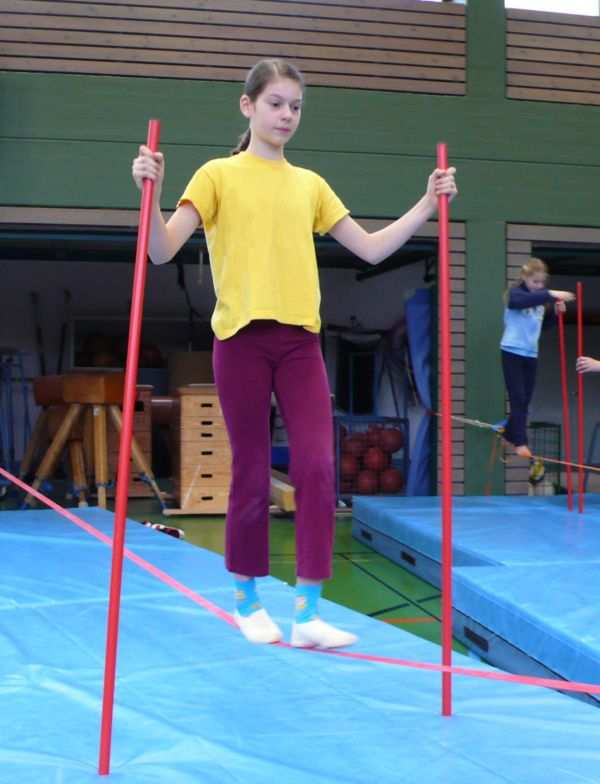
\includegraphics[width=1\linewidth]{Pictures/slacklineHelpSticks}
		\subcaption{Stick support}
		\label{fig:slacklineHelpSticks}
	\end{minipage}
	\hfill
	\begin{minipage}[t]{0.37\linewidth}
		\centering
		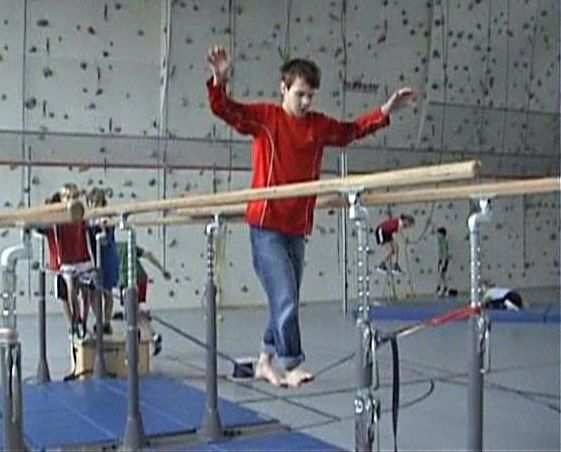
\includegraphics[width=1\linewidth]{Pictures/slacklineHelpBar}
		\subcaption{Between bars}
		\label{fig:slacklineHelpBar}
	\end{minipage}
	\hfill
	\begin{minipage}[t]{0.3\linewidth}
		\centering
		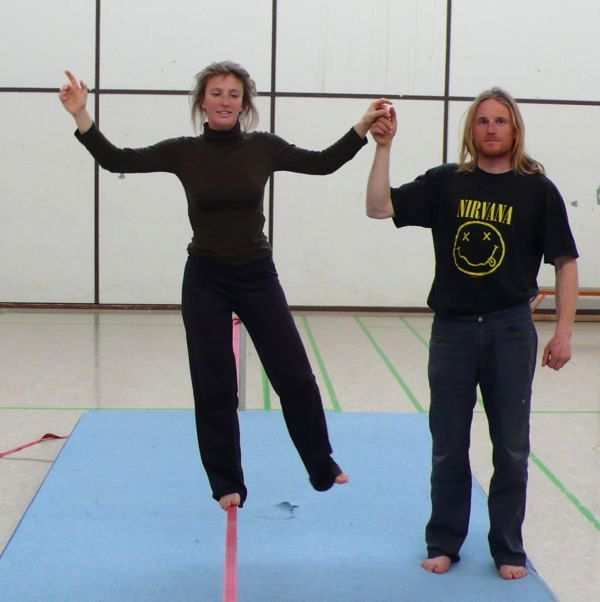
\includegraphics[width=1\linewidth]{Pictures/slacklineHelpHuman}
		\subcaption{Human support}
		\label{fig:slacklineHelpHuman}
	\end{minipage}
	\caption{Supportive exercises~\cite{Kroiss2007-ab}}
	\label{fig:supportiveExercises}
\end{figure}

With further progress, the external help should be reduced. The slacker can now try to stay and walk on the line on her own. It is recommended to begin with the practice of a basic start, to stay with both feet, and one feet on the slackline since these are basic techniques (Figure \ref{fig:basicExercises}). Staying with both feet seems easier in the beginning but only the hips and hands can be used for balancing. With just one feet on the line, the slacker can use the other one as an additional extremity for balancing purposes.
%For this one feet stays on the line and the other nearby on the ground. With a little swing the bodie's center of gravity should be brought over the slackline. A fundamental technique is to stay on one and both feet.

\begin{figure}[htb]
	\centering
	\begin{minipage}[t]{0.30\linewidth}
		\centering
		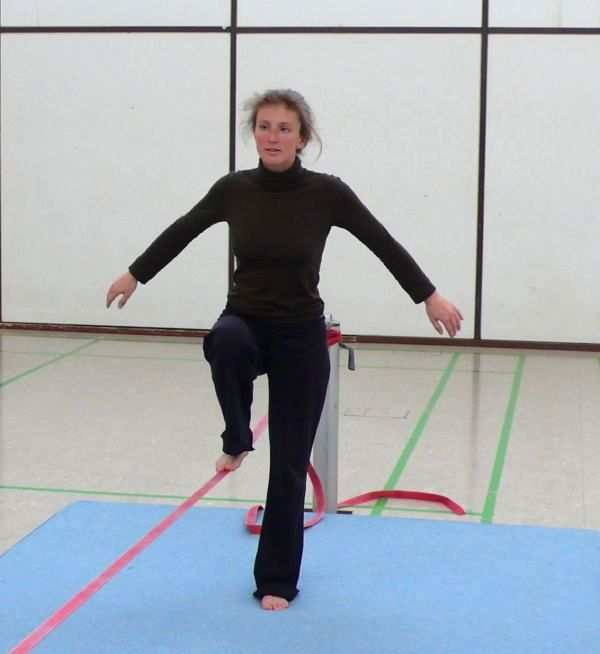
\includegraphics[width=1\linewidth]{Pictures/slacklineBasicStart}
		\subcaption{Basic start}
		\label{fig:slacklineBasicStart}
	\end{minipage}
	\hfill
	\begin{minipage}[t]{0.20\linewidth}
		\centering
		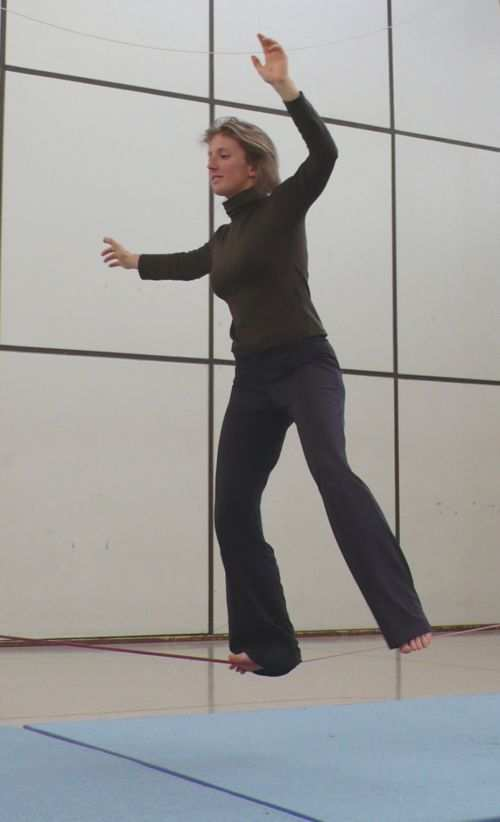
\includegraphics[width=1\linewidth]{Pictures/slacklineBasicOneFeet}
		\subcaption{One feet}
		\label{fig:slacklineBasicOneFeet}
	\end{minipage}
	\hfill
	\begin{minipage}[t]{0.33\linewidth}
		\centering
		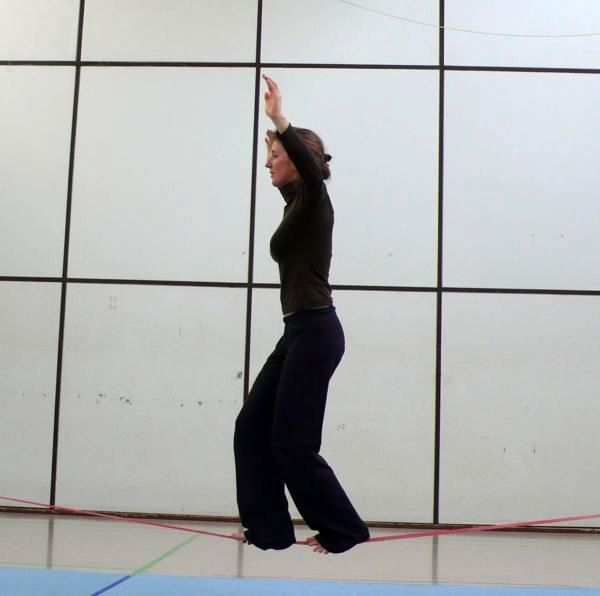
\includegraphics[width=1\linewidth]{Pictures/slacklineBasicBothFeet}
		\subcaption{Both feet}
		\label{fig:slacklineBasicBothFeet}
	\end{minipage}
	\caption{Basic exercises~\cite{Kroiss2007-ab}}
	\label{fig:basicExercises}
\end{figure}

Advanced training should be practiced in a more dynamical way~\cite{Thomann2013-aa}. Like seen in several research works~\cite{Donath2013-kk, Donath2016-gm, Granacher2010-ow, Keller2012-xh, Pfusterschmied2013-yy} this can be from crossover start (Figure \ref{fig:slacklineAdvancedCrossoverStart}), turning on the line, hands on hips or behind the back (Figure \ref{fig:slacklineAdvancedHandsBehindBack}), walk sidewards or backwards up to catch and pass a pall, kicking a football, bouncing a basketball, or a kneel down on the slackline (Figure \ref{fig:slacklineAdvancedDropknee}).

\begin{figure}[htb]
	\centering
	\begin{minipage}[t]{0.28\linewidth}
		\centering
		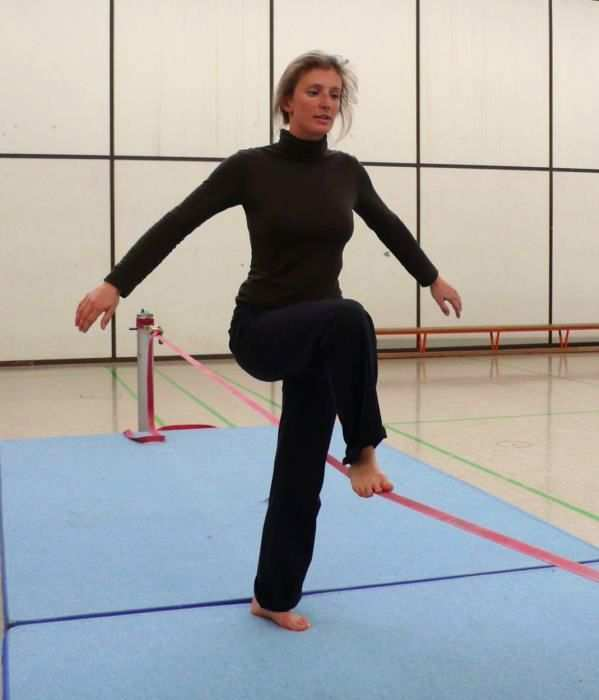
\includegraphics[width=1\linewidth]{Pictures/slacklineAdvancedCrossoverStart}
		\subcaption{Crossover start}
		\label{fig:slacklineAdvancedCrossoverStart}
	\end{minipage}	
	\hfill
	\begin{minipage}[t]{0.3\linewidth}
		\centering
		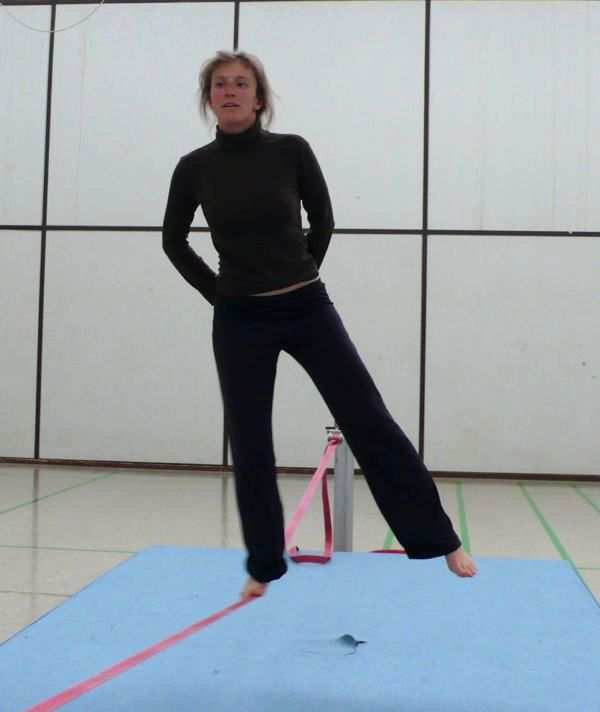
\includegraphics[width=0.9\linewidth]{Pictures/slacklineAdvancedHandsBehindBack}
		\subcaption{Hands behind back}
		\label{fig:slacklineAdvancedHandsBehindBack}
	\end{minipage}	
	\hfill
	\begin{minipage}[t]{0.38\linewidth}
		\centering
		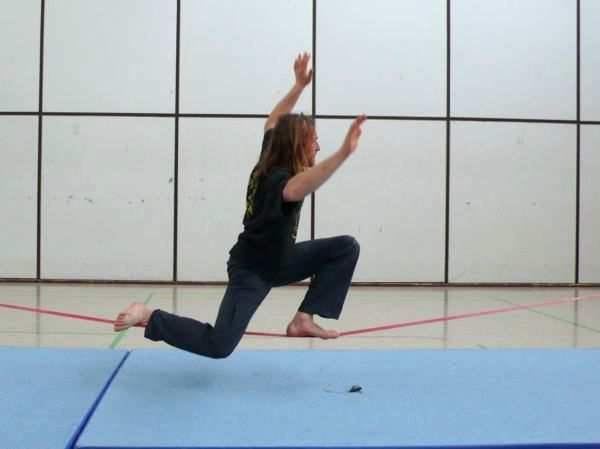
\includegraphics[width=1\linewidth]{Pictures/slacklineAdvancedDropknee}
		\subcaption{Dropknee}
		\label{fig:slacklineAdvancedDropknee}
	\end{minipage}	
	\caption{Advanced techniques~\cite{Kroiss2007-ab}}
	\label{fig:advancedExercises}
\end{figure}

Additional cognitive load is caused by unfamiliar exercises and simultaneous balancing on the line. This conjunction can lead to impairments. Even more difficult exercises can be carried out in further sessions like standing up from a sitting position, juggling, two people on the same line, reading a newspaper, closing eyes while balancing, vertical jumps, or rope skipping. Due to the higher difficulty of constraints, it results in a more unstable movement of the line.

Changes directly on the slackline itself, like varying the tension and length, have also an influence on the stability of the human body on the line~\cite{Keller2012-xh, Pfusterschmied2013-yy, Pfusterschmied2013-kq}. A short and tight line results in a relatively small vibrating area, where the slacker has to outbalance short unpredictable movements on point. Given a longer and loose line, it results in a more swinging behaviour that she has to counteract~\cite{Kroiss2007-ab}.
 
The slacklining assistance system should mainly train and support slacker to walk on the slackline. With those approaches in mind a foundation is set to build helpful exercises for the system. Because the focus relies especially on beginners, this information serves as an inspiration for supporting them with effective and efficient methods. Now is the question, what effect has slackline on the human body and where can it be applied? This is part of the next subsection.

\subsection{Slackline specific training effects and application scenarios}

Donath et al.~\cite{Donath2013-kk} elaborated the effects of slackline training on regular balancing, jump performance, and muscle activity with young children in school sport. The slackline specific balance has improved. Also the dynamic sway and muscle activity for the lower limb is reduced. But there were no effects regarding jump performance. The children enjoyed the slackline training. In comparison to classical balance training it can be more fun for the children and at the same time an effective training method.

Another study of Donath et al.~\cite{Donath2016-gm} investigated slackline training with seniors from an age between 59 to 69 to measure effects on slackline specific balance and neuromuscular performance. They found significant differences between pre- and posttests during all slackline stance conditions. In addition the trunk and limb muscle activity were reduced after the training phase. With this in mind slacklining can be provided as an alternative balance training method for seniors. Regular balance training can help to reduce the fall risk, which can be an useful therapy for seniors when keeping in mind that 30\% of seniors suffer from fall injuries once a year.

Keller et al.~\cite{Keller2012-xh} examined the improvement of the postural control regarding the Hoffmann-Reflex after slackline training and whether adaptations can be found regarding classical balance training. The H-Reflex (Hoffmann-Reflex) is used to assess and quantify stretch-reflex responses due to electrical stimulation. The measurements show that these were significantly reduced as well as slackline specific balance were improved. Therefore slackline training and classical balance training have at least similar effects on the postural control.

Pfusterschmied et al.~\cite{Pfusterschmied2013-yy} found significant effects regarding stable stance after slackline training and even more effects were found for perturbed leg stance. This is because slacklining is a high dynamic movement activity and there is more need of regaining equilibrium as in perturbed stance than for maintaining balance as in a stable leg stance condition. The velocity in medio-lateral and anterior-posterior center of gravity, knee and hip joint is reduced as well as the range motion in knee and hip joint. No changes in medio lateral direction for the stable surface or joint kinematics for both have been found.

Another study of Pfusterschmied et al.~\cite{Pfusterschmied2013-kq} shows effects on lower limb joint motion and muscle activation. They found a decrease in platform velocity and improvements in corrective action in the knee joint. Also enhanced activation of the muscle activity in rectus femoris (upper leg) was measured.

Granacher et al.~\cite{Granacher2010-ow} investigated the impact of slackline training for balance and strength promotion and found contradictory results compared with the studies described above. Static and dynamic postural control were analysed as well as the isometric and dynamic muscle strength. There were no effects regarding the postural control, maximal torque, and jumping height. The results can be explained due to the assessment of other recorded variables, usage of different methods for analysing the data, and the relatively short slackline training time than in other studies~\cite{Pfusterschmied2013-yy}. Therefore this study can be seen as an exceptional case.

Those investigations show that slacklining is indeed an effective method for improving the postural control. Hence many application scenarios can be thought of to implement a slacklining assistance system. For example it can be used as a training approach in school sport, preventative activity for seniors, and rehabilitation alternative. Furthermore it can be used as a supportive training method for athletes in sport activities like skiing or skating, that require a good body balance. Interactive technologies can be used to support training in such scenarios. The next section provides an overview about state of the art technologies, compares them, and show several implementations in balance scenarios.
\newpage

\section{Interactive technology}\label{2_3_interactiveTechnology}

To build a real time feedback assistance system, a tracking device is needed that supports the slacker in an appropriate way and won't interrupt her. The Microsoft Kinect v2 seems like a suitable tracking system in this context, because the user don't need any further devices to be tracked. But it should be compared with other tracking technologies like the Nintendo Wii, Playstation Move, and a motion control suit, to justify its usage. In the following advantages and drawbacks of these systems will be discussed. Further several studies show how accurate and precise the Microsoft Kinect v2 is, if it can be applied for balancing purposes, give the user appropriate feedback, or useful analysis data for specialist like therapist.

\subsection{Comparison of tracking technologies} \label{trackingTechnologie}

The Nintendo Wii consists of a sensor bar with infrared sensors that estimates the position of the Wiimote controller in 3D. Further an accelerometer is integrated in the Wiimote to detect its motion. Thus the user can interact with the console, based on predefined gestures~\cite{Bogdanovych2015-ci, Tanaka2012-ACO}. Gesture recognition is an essential aspect of the slacklining assistance system for giving appropriate feedback regarding the executed exercise. Schlömer et al.~\cite{Schlomer2008-uo} analysed the gesture recognition of the Wii and found an error rate between 5\% and 15\%.

A similar approach with a handheld controller is followed by the PlayStation Move. It contains an RGB camera called Move Eye that is used for tracking the 3D position of a lighting sphere attached on the handheld device named Move wand. The controller contains an accelerometer, gyro sensor and geomagnetic sensor to track the rotation and also support position tracking. In this way more accurate tracking is possible than with the Nintendo Wii~\cite{Bogdanovych2015-ci, Tanaka2012-ACO}.

Both systems are good devices if the controller itself can be replicated as a virtual device like for example in golf or tennis. But they do not track the body movement and the user is bound to her handheld devices to interact with the system. In the slacklining system they could disturb user standing on the slackline. Moreover accurate feedback from the whole body is wanted and thus it should be the actual controlling device. Therefore they seem not to be appropriate devices for the slacklining system.

With a motion capture suit markers have to be attached on the user’s body for tracking her body motion and rotational data. This makes it the best device for high accuracy and precision body tracking. Problems with the suite are that it is very expensive and the setup takes relatively long time because of the marker attachment and the positioning of the tracking cameras. The biggest drawback is the uncomfortable bulky equipment that could interfere the user during the performance~\cite{Bogdanovych2015-ci, Chang2012-hz, Nusman2006-rf}. This makes it an inappropriate device for user tracking on a slackline.

The Microsoft Kinect is a static device that includes a RGB camera and depth sensor. Because the body joints and player position are recognised by these, the user is free in her movement without any further controller. Another advantage is the low price in comparison to the motion control suite, and the low setup time because only the device itself is needed. Problems occur with occlusion of body parts that results in glitches and flawed tracking~\cite{Kajastila2014-ug, Tang2015-wt}. To the user they can be hidden, e.g. by only showing the output of the depth cam~\cite{Holsti2013-kn}. This problem can also occur in the slacklining case because of overlaying feet. Therefore a feasibility study should be realised to show if this is a bigger problem or can be neglected. 
%The results can be seen in section \textbf{<NUMBER>}. 

With this in mind, the Microsoft Kinect v2 seems like the most suitable device. The recognition of the whole body, freedom of movement, short setup time, and relatively low cost makes it the best system out of the stated devices.

\subsection{Accuracy of the Microsoft Kinect}

In the field of balance training it is necessary to give appropriate feedback for the patient that reveals errors in the performance and support a proper execution. With this in mind user tracking should be good enough to fulfil this criteria. Since Microsoft Kinect is used as the tracking device the accuracy and precision should be assessed.

Lim et al.~\cite{Lim2015-pw} assessed the accuracy of the Kinect with a 3D motion capture system as a reference system. For further understanding please review Figure \ref{fig:bodyWikiAnatomicalTermsOfLocation} regarding expressions to body planes and anatomical directional references. The participants had to execute balance training with complex aperiodic movements in the body planes (Figure \ref{fig:bodyPlanes}). Similar characterization of movements are provided by the Kinect in comparison to the 3D motion capture system. The correlation analysis showed that the Kinect and the 3D motion capture system are highly correlated for the flexion and extensions in the medio-lateral-axis (x-axis) but not on the anterior-posterior-axis (y-axis) and the cranial-caudal-axis (z-axis) (Figure \ref{fig:bodyDirectionalReferences}). This is because the Kinect determine joint locations based on the depth image data and the data input is limited to the depth camera view. Therefore recognition of joint angles in the sagittal and transverse plane is not optimal (Figure \ref{fig:bodyPlanes}). Also the primary goal of the Kinect is to measure the dynamic movements in the coronal (frontal) plane for gaming reasons. It is indeed an effective system to characterize changes in center of mass and movements in the frontal plane during balance training. But it would not be suitable in balance training that require in-depth analyses of joint motions, which is not needed with the slackline assistance.

\begin{figure}[htb]
	\centering
	\begin{minipage}[t]{0.38\linewidth}
		\centering
		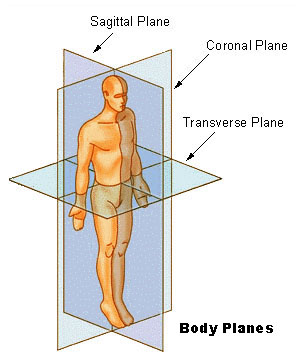
\includegraphics[width=1\linewidth]{Pictures/bodyPlanes}
		\subcaption{Body Planes}
		\label{fig:bodyPlanes}
	\end{minipage}
	\hfill
	\begin{minipage}[t]{0.6\linewidth}
		\centering
		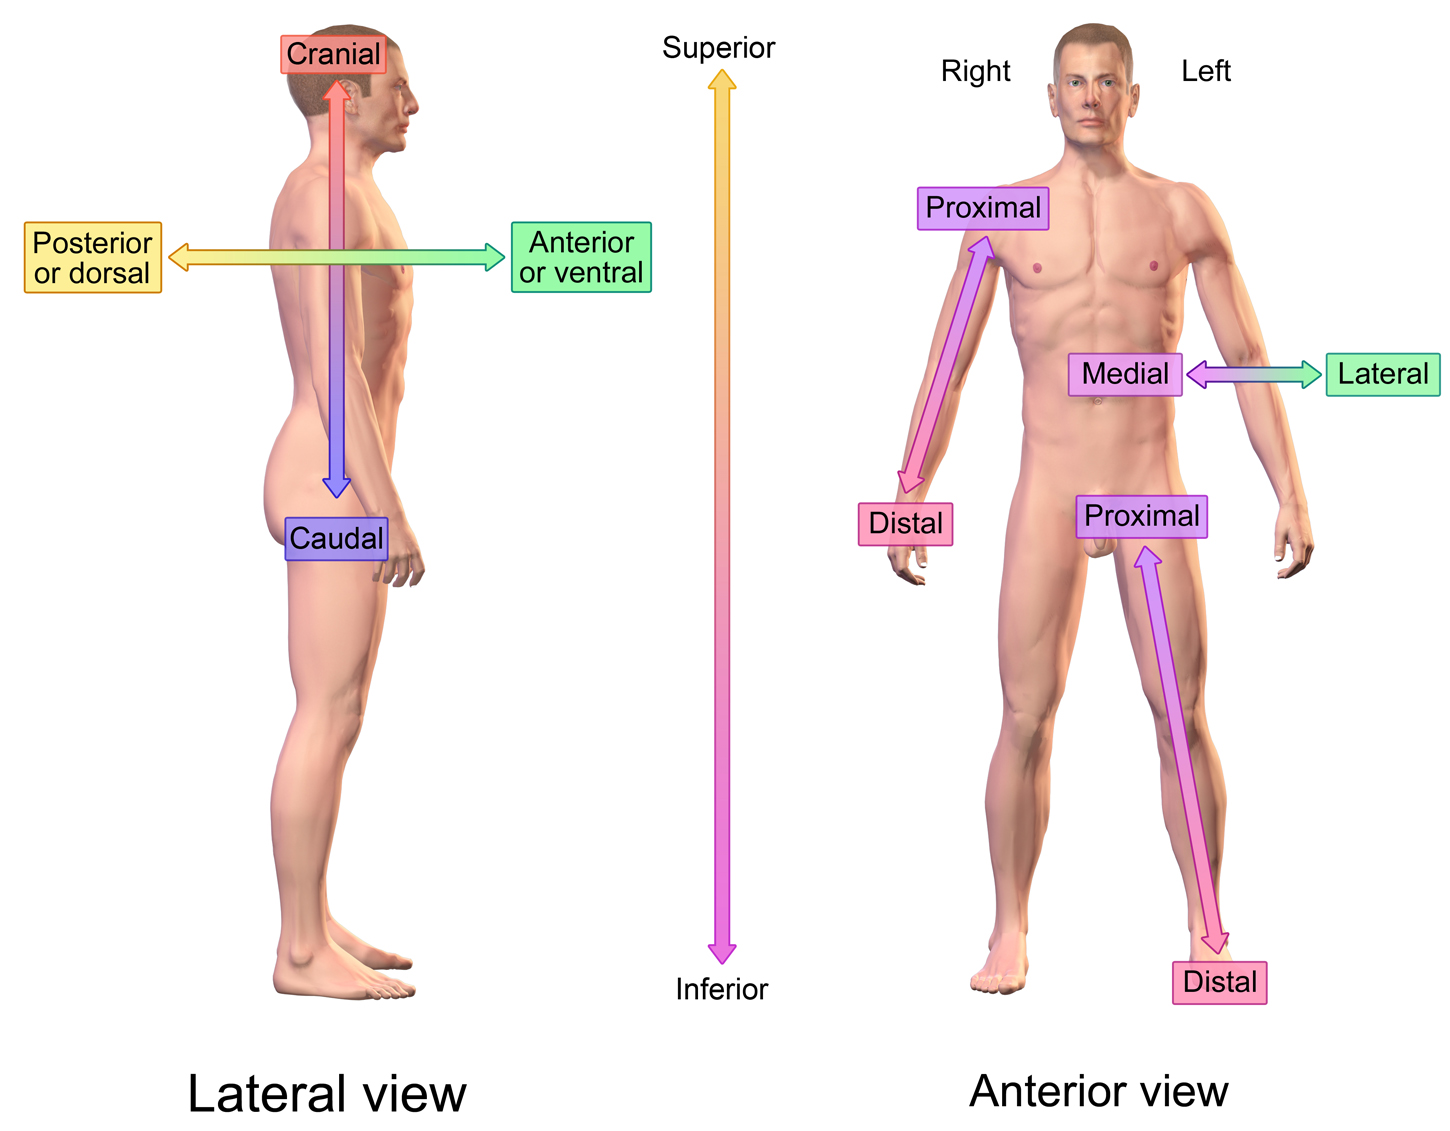
\includegraphics[width=1\linewidth]{Pictures/bodyDirectionalReferences}
		\subcaption{Directional References (modified)}
		\label{fig:bodyDirectionalReferences}
	\end{minipage}
	\caption{Anatomical terms of location~\cite{Wiki2017-ATOL}}
	\label{fig:bodyWikiAnatomicalTermsOfLocation}
\end{figure}

Chang et al.~\cite{Chang2012-hz} focuses mainly on the tracking performance of the Microsoft Kinect as a rehabilitation device in comparison with a high fidelity motion capture system called OptiTrack. In their application the user has to move objects from one side of the screen to the other. Five correct and incorrect movements have been realised and both systems successfully identified them. In trajectory comparison the results of the hand and elbow by the Kinect are very close to the OptiTrack system. Tracking of the shoulder movements are moderate because it involves rotation that the device does not recognizes well. The timing performance comparison shows that the OptiTrack system is negligible faster than the Kinect.

Woolford~\cite{Woolford2015-ub} compared the accuracy and precision of the Kinect v2 with the Qualisys motion capture system for the usage in healthcare applications. He describes that accuracy is the amount of how close a measured quantity to the actual value is. Precision is the similarity of repeated measurements (Figure \ref{fig:systemAccuracyAndPrecisiong}). For example the Kinect skeleton tracking methods are accurate because the average joint position data is very close to the actual physical position. Regarding his definition of precision, the joint position data is not always precise because the data spreads in its position of the frame. The results show that the Kinect V2 is accurate but imprecise for body parts whose center of mass cannot be easily identified like the shoulder. For smaller body parts as well as between two body parts such as elbow or wrist the accuracy and precision is very high. 

\begin{figure}[htb]
	\centering
	\begin{minipage}[t]{0.49\linewidth}
		\centering
		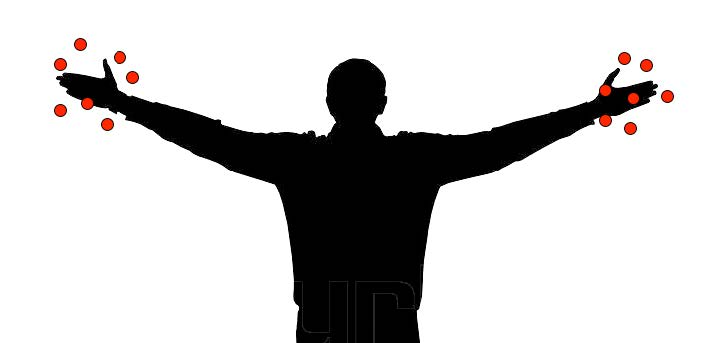
\includegraphics[width=1\linewidth]{Pictures/systemInaccurateImprecise}
		\subcaption{Inaccurate and imprecise system generates random-like measurements}
		\label{fig:systemInaccurateImprecise}
	\end{minipage}
	\hfill
	\begin{minipage}[t]{0.49\linewidth}
		\centering
		
\includegraphics[width=1\linewidth]{Pictures/systemInaccuratePrecise}
		\subcaption{Inaccurate but precise system, where measurements are close to each other but have systematic error}
		\label{fig:systemInaccuratePrecise}
	\end{minipage}
	\hfill
	\begin{minipage}[t]{0.49\linewidth}
		\centering
		
\includegraphics[width=1\linewidth]{Pictures/systemAccuratePrecise}
		\subcaption{Accurate and precise system generates measurements that are close to the real world}
		\label{fig:systemAccuratePrecise}
	\end{minipage}
	\hfill
	\begin{minipage}[t]{0.49\linewidth}
		\centering
		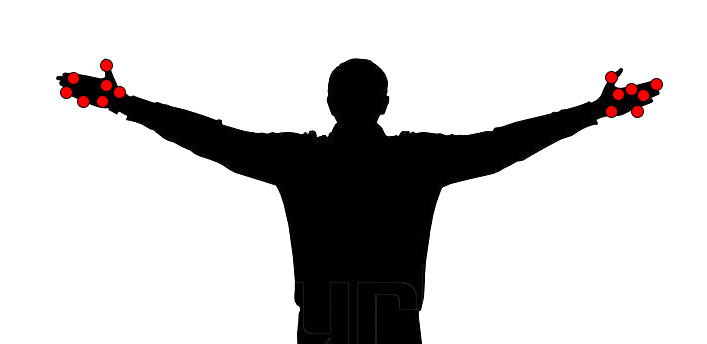
\includegraphics[width=1\linewidth]{Pictures/systemAccurateImprecise}
		\subcaption{Accurate and suffice precise system generates measurements that are close to each other and are not systematically biased}
		\label{fig:systemAccurateImprecise}
	\end{minipage}
	\caption{Definition of accuracy and precision~\cite{Woolford2015-ub}}
	\label{fig:systemAccuracyAndPrecisiong}
\end{figure}

The Microsoft Kinect v2 can indeed be compared with high performance tracking devices. If no detailed analysis is needed, it provides reliable and appropriate data. For the assistance system it should provide sufficient data to track the user and give useful feedback

\subsection{Implementation in balance training scenarios}

Like already stated Chang et al.~\cite{Chang2012-hz} not only assessed the accuracy of the Microsoft Kinect but also if it could fit as an alternative training device in rehabilitation training. The results show that it provides enough usable feedback to the therapists to be an appropriate device for medical uses. Woolford~\cite{Woolford2015-ub} state that the Microsoft kinect is a useful device for monitoring such exercises. The set-up is relatively easy and the tracking is appropriate for exercises in a healthcare environment. Lim et al.~\cite{Lim2015-pw} investigated the usage of Microsoft Kinect in the field of falling risk. They tracked characterizing movements and found that it is an useful device for balance training. Ustinova et al.~\cite{Ustinova2014-ml} used the Kinect to improve the postural control as well as coordination deficits from chronic traumatic brain injury patients. It resulted in improvements of postural stability, movement performance and motoric coordination. The participants were also very satisfied whereas normal exercises have been stated as boring. Pisan et al.~\cite{Pisan2013-sf} used the device to investigate the prediction of the loss of balance for elderly users with a step training program. The user preferred doing exercises with the system and the tests matched also the expectation of the researcher. An integration in promoting the postural control for parkinson disease with 

Kinect games were elaborated by Pompeu et al.~\cite{Pompeu2014-yl, Pompeu2015-vp}. The results affirm that the patients improve in balance purposes and motoric movements with this help.

Furthermore Estapa et al.~\cite{Estepa2016-oj} and Freitas et al.~\cite{Freitas2012-ae} collected data of execution from patients for medical reviews. Both developed a motor rehabilitation game. It is used to support therapeutic exercises and evaluate biomechanics of the patients. This allows subsequent analysis of the performance data for the therapist.

This approach of data analysis was also integrated by Garrido Navarro et al.~\cite{Garrido2013-zs} but in addition they elaborate if the Kinect can serve as a rehabilitation home assistance. Many patients are thrown out of their daily life environment for accessing traditional rehabilitation training in a medical center. Here the patient incorporate the system into their daily life and avoid such trips. The medical stuff gets all relevant parameters due to the transmission of the recordings from the exercises to the medical center. Beside this they get more time because nobody has to observe the training.

Keeping the stated results in mind shows that the Microsoft Kinect is a promising system for balance exercises that provides sufficient accurate and usable feedback. It can be embedded in a variation of fields as rehabilitation system, home assistance, or preventative technique. The aspect to motivate patients with an exergame approach and enjoyable user interface can also lead to successful exercise execution, which is part of the next section.
\newpage

\section{Feedback and interaction methods}

Cognitive load plays an important role if skill acquisition is a major factor. In slacklining the user has to focus on multiple things simultaneously that increases the mental pressure. Several studies show why and how the cognitive load should be restricted. Another important fact is that repetitive exercises can lead to a boring and demotivating user experience. For that reason several methods, systems and game approaches can be used as an inspiration to build a system with a motivating and joyful environment. At last the integration and visualisation of feedback and interaction methods should be well thought out. Various techniques have been elaborated on how to provide this appropriately.

\subsection{Restricting cognitive load}

As a baseline Paas et al.~\cite{Paas2003-xt} describes that the acquisition of new skills is in conjunction with cognitive load. By adjusting this the learning effect can be easened or hardened. Three types of cognitive loads exists that handle the working memory of a person regarding the learning process. Intrinsic load is the inherent complexity that is caused by the topic itself. It is also important in which manner information is given to the user. If this is unnecessary, repetitive, or interferes her it is called an extraneous cognitive load and increases the burden of the user. The last type is germane cognitive load, which describes also how information is given to the user but by supporting the him in that way. This is brought by activating and automating already existing patterns or generating new ones in the working memory to enhance a learning process. Regarding this several applications have been evaluated that are also relevant to the slacklining supporting system.

Van der Spek~\cite{Van_der_Spek2010-fe} evaluated how to deal with the right complexity in serious games. He describes in his mental model construction (Figure \ref{fig:mentalModelConstruction}) that interference can be avoided by information regulation and focus attention. Improving is encouraged by predictability and reflection of the tasks. The attention of the user should be focused to relevant material by regulating the information given to him. Since a serious game like approach should be developed this is an important reference for building an effective learning process to the user.

\begin{figure}[htb]
	\centering
	\begin{minipage}[t]{0.8\linewidth}
		\centering
		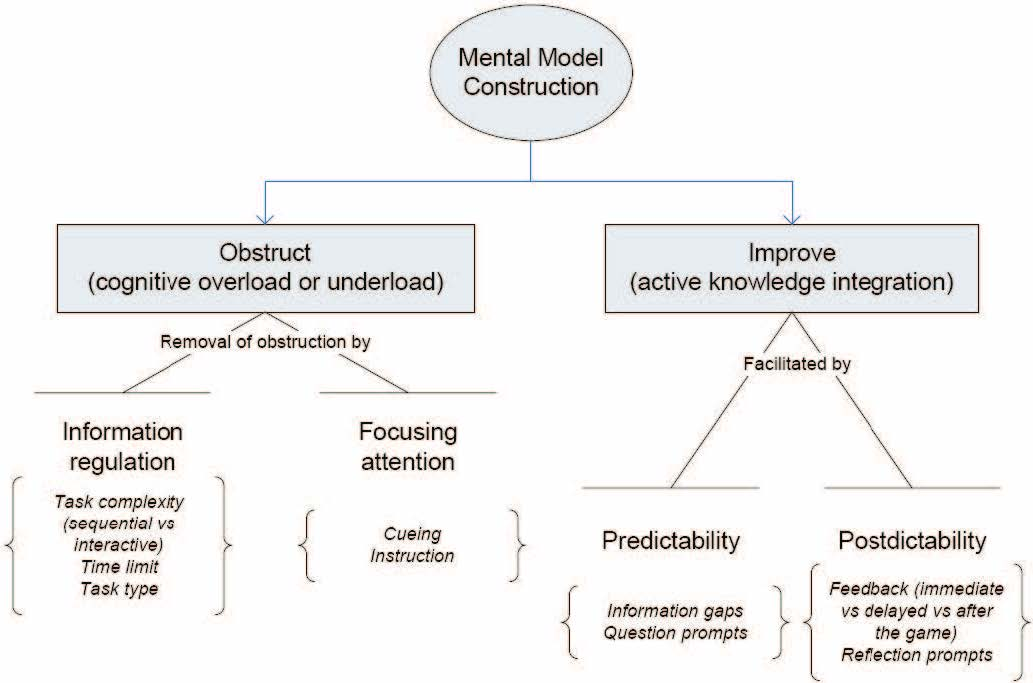
\includegraphics[width=1\linewidth]{Pictures/mentalModelConstruction}
		\caption{Guideline for enhancing the cognitive load~\cite{Van_der_Spek2010-fe}}
		\label{fig:mentalModelConstruction}
	\end{minipage}
\end{figure}

Pisan et al.~\cite{Pisan2013-sf} evaluates the user risk of falling with cognitive loading exercises. They executed two stroop tests, where the participant had to name the correct color of the word. High and low cognitive load can be measured by differentiating the meaning and color of a word. In the next challenge she has to answer different maths problems provided by the system. The results show that the reaction time due to cognitive load is much larger with users that have a higher risk of falling than for users that have a lower risk. This could be explainable due to the fact that user with higher falling risk are not that good in terms of switching the cognitive focus from the balancing action into other actions. 

Training on a slackline provides cognitive load to the user because of several simultaneously things she has to be aware of. Hence feedback given on how to behave in a situation should be provided in an appropriate manner to support the slacker. The system has to be aware of this and restrict the cognitive capability in the right way. Next to cognitive load the system has to ensure that the user stays motivated for the training, which is part of the following subsection.

\subsection{Motivating factors for skill acquisition}

Several rehabilitation and sport training programs can be elaborated for motivating facotrs because the skill acquisition in slacklining resemble with them. The training procedure is a process of repetitive exercise execution. For mastering new skills and extend himself a user must have the willingness and commitment for practicing, which can be described as motivation. The self-determination theory by Ryan et al.~\cite{Ryan2000-jn, Ryan2000-gi} describes several types of motivational factors. First the intrinsic motivation, which is caused by interest to an action and satisfies the own psychological needs for self-determined behaviour. This is the fundamental stimulus for high valuable learning and practicing. Second the extrinsic motivation that is performing an activity because of an external output. The user can hereby feel externally propelled due to compliance with external regulations or she can be self-endorsed due to willingness and acceptance by the value of the practice. 

Johnson et al.~\cite{Johnson1998-hb} stated regarding rehabilitation training that if exercises and the user himself provide negative factors like boredom, repetition or long execution time it results in a discouragement. Enhancing the interaction with this trainings can lead to effective training. 
Pisan et al.~\cite{Pisan2013-sf} says that video games can help to motivate the patients through their physical training. The participants in his user tests found the games that he developed engaging. They preferred doing the exercises with the system.

Several researchers involved the motivational aspect of video games in their system. Ustinova et al.~\cite{Ustinova2014-ml} developed four custom virtual video games to elaborate the efficacy for postural deficits. First a virtual teacher where the subject has to copy its movements strictly. Second a virtual challenger that is divided into a skateboard, courtyard and an octopus game with specific exercises in which the movements of the user are more flexible. Successfully completed performance will be rewarded with a number of points. Overall the user were strongly satisfied with the gaming part of the therapy and moderate with the virtual teacher part.

Freitas et al.~\cite{Freitas2012-ae} focused on user centred development of a physiotherapeutic game that supports motor rehabilitation exercises. A plane represented the user and she has to fly through rings in the air and avoid obstacles. The patients were strongly satisfied with the game. An important factor here is the good user interface that affects the user motivation, visually presented scenario and playing technique in a positive way.

Estepa et al.~\cite{Estepa2016-oj} evaluates three developed exergames involving different psychophysical rehabilitation exercises. A virtual avatar represents the patient and orders are giving via an auditive or visual stimuli. The first two games are a series of coming balls placed at desired angles that the patient has to avoid with her trunk or, in the second game, with her feet. In the third exercise she has to step forward to a colored line between starting and goal position. All games were easy to understand and provide necessary feedback. The patients had a considerable interest to use the system.

Kajastila and Hämäläinen~\cite{Kajastila2014-ug} encourages monotonous parts of climbing training by adding goals and supporting the social collaboration of the participants. Hence they are making it overall more enjoyable. Six prototypes were developed. Prototypes that rely more on a training part are an easy route builder, automatic route generator and instant video feedback. For the user those were the most useful ones. The exercises that consists of a more playful part, such as a chasing animated saw that the climber has to avoid, shifted the focus away from the training part. 

With this in mind an useful training device should be considered that includes an enjoyable virtual environment. A good balance between these both is the key for successful and motivating skill acquisition. Another part of the system should also provide useful feedback to the slacker. Which methods can be used for this will be discussed in the following.

\subsection{Approaches and techniques for providing feedback}

Several technological advances like video feedback, virtual environments and auditive information can be applied for providing feedback in sport activities. Liebermann et al.~\cite{Liebermann2002-zr} evaluated those regarding their field of application. With video information costs are relatively low, it is easy accessible, and portable. It can be repetitively replayed in real-time or superposition of two video. Training in 3D virtual environments can help to improve or to familiarize with a real world skill acquisition. The user can pre-practice a skill in simulated unknown conditions like pilots in a simulated airplane. Providing appropriate auditive information can also have a relatively high impact on performance enhancement. Also the Microsoft HCI-Guidelines state that implementing audio is a good way if the user need to be notified, and to indicate states of changing behaviour~\cite{MicrosoftHIG2014-mh}. For example in balance training a warning signal can indicate that the current pose is not the desired one. If the user corrects his posture in the right way, the signal should then transform into an more comfortable signal. All of these allow qualitative and meaningful feedback in their application context. The user can review the execution, pre practice in a virtual environment, or be supported by audio warning signals. WIth this she can discover failure in her performance.

Feedback has to be provided in an appropriate manner for improving new motor skill acquisition. Especially for starting to learn a new technique it is important to have immediate feedback sources on which the user can rely on~\cite{Hodges2002-gb, Winstein1990-to}. Therefore it should be easy to understand for enhancing the learning process. 

Hämäläinen~\cite{Hmlinen2004-ai} developed applications for a camera output in front of the user. An automated motion controlled approach starts and stops the recording if the motion exceeds a certain threshold. Second a speech and last a gesture control prototype. Both consists of four commands to record, play, stop and delay the recording. The user test ranked the automatisation the worst because it reacted to unintentional motions, which ends in unwanted command recognition. The speech system ranked the best but only worked well if the participant speaks near the microphone. Some mentioned that the gesture approach were more intuitive and natural, which could be a good compromise out of the three approaches.

Holsti et al.~\cite{Holsti2013-kn} investigated delayed video feedback and a platform jumping game in trampoline sport. The former records the performance execution and shows it repetitive to the user. In the second the player has to jump back- and forwards on virtual platforms. They tested it with athletes and beginner. The delayed video feedback was ranked useful for nearly all athletes. Overall the platform jumping game was ranked the best.

Kajastila and Hämäläinen~\cite{Kajastila2014-ug} project graphics on an artificial climbing wall. A feasibility study showed that graphic information is best located near holds where the focus of the climber goes naturally. 
This can be adapted to slacklining since the slacker has to focus usually a specific point in front of her.It would be useful to provide information in the peripheral view. Next to other prototypes he has implemented an instant delayed video feedback. This is rated as one of the most useful ones because the user can immediately analyse her performance. Also a gaming approach is developed as an animated saw that chases the climber and has to be avoided. User state that it moves the focus away from the training, but it could be an enjoyable alternative to kids for getting them used to the sport. 

Based on the results of the last paper Kajastila et al.~\cite{Kajastila2016-ot} developed two games and a route creation application. User emphasize the versatility and excitement of the games. They also forget the fear of heights due to time limits and forcing them to focus and achieve a goal. User stated that playing and spectating is also more fun due to implemented sound and visual effects.

Like seen a delayed video feedback is a good approach to learn new skills. Combining this with a gaming approach can simultaneously lead to a joyful experience with training aspects. Also adding audio signals can further improve this experience for the user as well as for spectators. A well suited interaction mechanism and a good looking environment can help to create an effective system and motivate the user for training purposes.

\subsection{User interface}

Important feedback information during the exercise should be placed surrounding the focus point in the peripheral view of the user. Directing the user for correcting her movement can be done in several ways. Basic information about the execution should be given prior to the user for exercise preparation. Surrounding objects can be displayed as arrows, flashing notifications or weighting scale like seen by Garrido Navarro et al.~\cite{Garrido2013-zs} in Figure \ref{fig:informationUISurroundingObjects}. Additional informations like current exercise and the state can be displayed outside of the focus space. But they should be designed to not distract the user. If they do so it should be able to just show the feedback visualisations. A feedback summary after the execution can give an useful resume about the exercise as an reflection like in Figure \ref{fig:informationUIFeedbackSummary}.
\begin{figure}[htb]
	\centering
	\begin{minipage}[t]{0.46\linewidth}
		\centering
		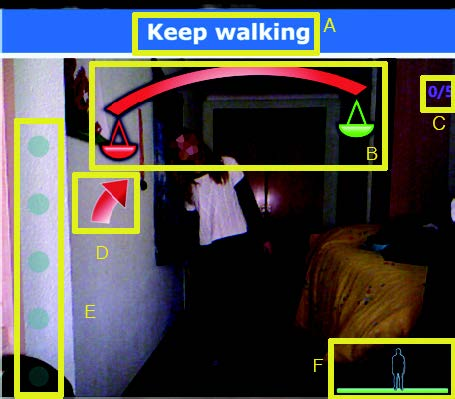
\includegraphics[width=1\linewidth]{Pictures/informationUISurroundingObjects}
		\subcaption{Surrounding objects in the UI}
		\label{fig:informationUISurroundingObjects}
	\end{minipage}
	\hfill
	\begin{minipage}[t]{0.46\linewidth}
		\centering
		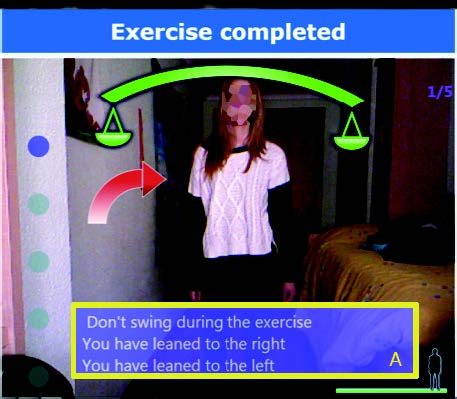
\includegraphics[width=1\linewidth]{Pictures/informationUIFeedbackSummary}
		\subcaption{Completed exercise feedback summary}
		\label{fig:informationUIFeedbackSummary}
	\end{minipage}
	\caption{Interface of a rehabilitation training application~\cite{Garrido2013-zs}}
	\label{fig:informationUIGarrido}
\end{figure}

Another method is to show the user itself or an avatar that demonstrates the correct performance of the current exercises like in Figure \ref{fig:avatar3DModel} and \ref{fig:avatarUser}. Holsti et al.~\cite{Holsti2013-kn} implemented such a user integration and in user testing they endorse to see themself performing in real time.

\begin{figure}[htb]
	\centering
	\begin{minipage}[t]{0.49\linewidth}
		\centering
		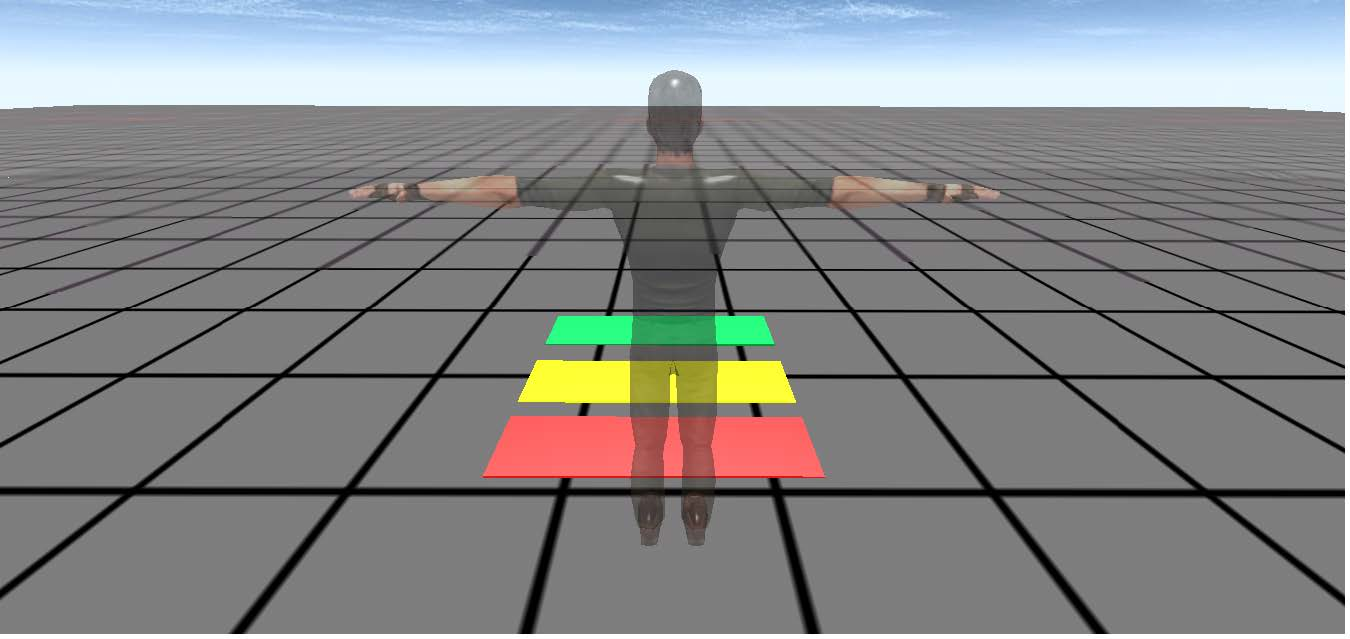
\includegraphics[width=1\linewidth]{Pictures/avatar3DModel}
		\caption{3D Model as avatar~\cite{Estepa2016-oj}}
		\label{fig:avatar3DModel}
	\end{minipage}
	\hfill
	\begin{minipage}[t]{0.49\linewidth}
		\centering
		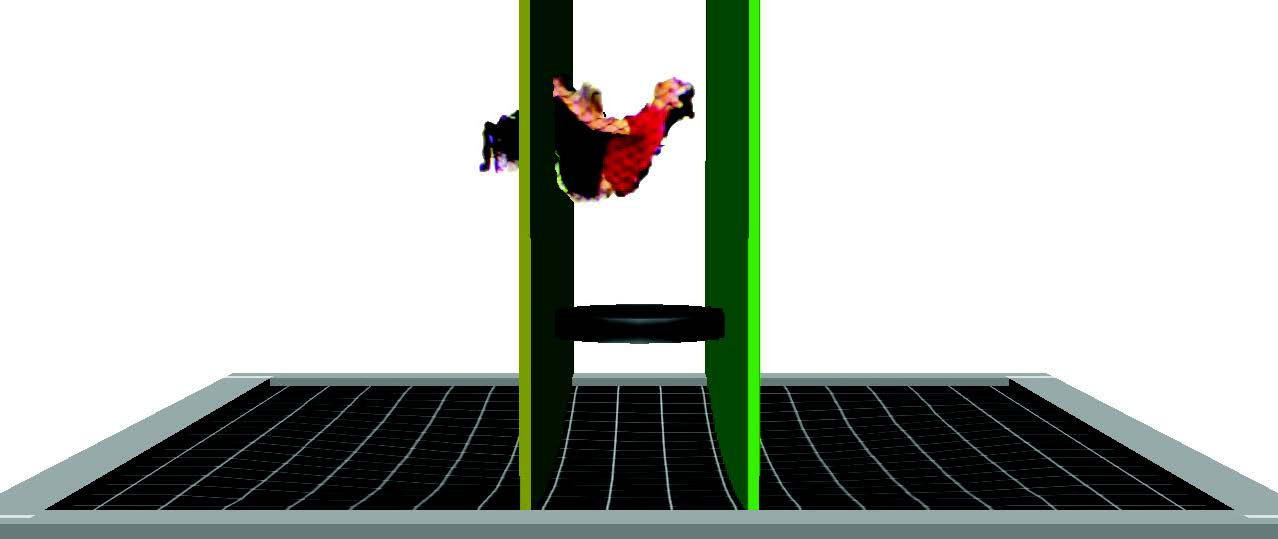
\includegraphics[width=1\linewidth]{Pictures/avatarUser}
		\caption{Rail-time user representation~\cite{Holsti2013-kn}}
		\label{fig:avatarUser}
	\end{minipage}
\end{figure}

The task about the execution has to be clarified. Chang et al.~\cite{Chang2012-hz} provides real time feedback on the performance quality due to a visualised path. If the performance is correct the path will turn green. But if she moves outside the range the path turns red and an arrows guides him into the correct position. Instructions and highlighting objects can help to complete an exercise successfully (Figure \ref{fig:gameUIChang}). If she performs something wrong during the performance e.g. in the slacklining case corresponding body parts could be highlighted.

\begin{figure}[htb]
	\centering
	\begin{minipage}[t]{0.49\linewidth}
		\centering
		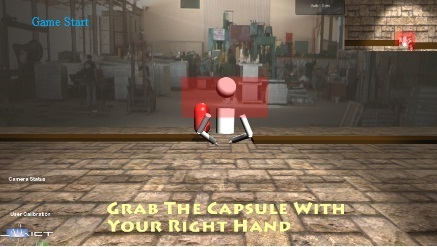
\includegraphics[width=1\linewidth]{Pictures/gameInstruction}
		\subcaption{Instruction to the game}
		\label{fig:gameInstruction}
	\end{minipage}
	\hfill
	\begin{minipage}[t]{0.49\linewidth}
		\centering
		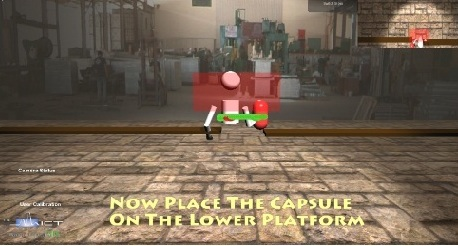
\includegraphics[width=1\linewidth]{Pictures/gameHighlighting}
		\subcaption{Green indicator for correct performance}
		\label{fig:gameHighlighting}
	\end{minipage}
	\caption{User interface of a rehabilitational application~\cite{Chang2012-hz}}
	\label{fig:gameUIChang}
\end{figure}

Microsoft itself offers human interface guidelines for the Kinect v2~\cite{MicrosoftHIG2014-mh}. In this document is describes how to design and develop for the user. It provides a quick introduction into the Kinect itself, design principles for interactions regarding gesture and voice, and how to visualize appropriate feedback. Also which interactions should be used for a specific action. Overall design principles are that the application should be context-aware, make the user confident, choosing the right input method and to conduct user tests. A gesture that relies on the real world can help the user to be more familiar with the product, than learning unknown gestures (Figure \ref{fig:hciGuidelinesDynamicGesture}).

Teaching gestures is a core functionality in the slacklining assistance system. The HCI-Guidelines state that new gestures should be teached with a quick tutorial. Further a visual hint, animation, or notification can also help for first the engagement (Figure \ref{fig:hciGuidelinesTeachingMethods}).
\begin{figure}[htb]
	\centering
	\begin{minipage}[t]{0.45\linewidth}
		\centering
		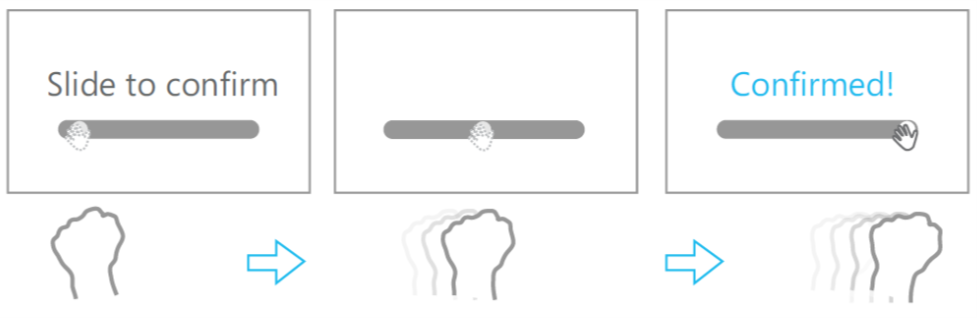
\includegraphics[width=1\linewidth]{Pictures/hciGuidelinesDynamicGesture}
		\subcaption{Slider as dynamic gesture}
		\label{fig:hciGuidelinesDynamicGesture}
	\end{minipage}
	\hfill
	\begin{minipage}[t]{0.45\linewidth}
		\centering
		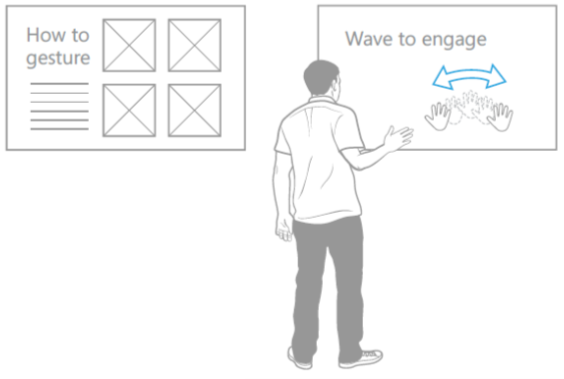
\includegraphics[width=0.8\linewidth]{Pictures/hciGuidelinesTeachingMethods}
		\subcaption{Teaching new gestures}
		\label{fig:hciGuidelinesTeachingMethods}
	\end{minipage}
	\caption{Gesture interaction~\cite{MicrosoftHIG2014-mh}}
	\label{fig:hciGuidelinesMicrosoft}
\end{figure}

Appropriate feedback should visualise if the sensor is ready, the user is visible to the Kinect, she is engaging right now, etc. For example if the user can control something with his hand can be visualised in form of a cursor and the state of a UI control element should also be clear (Figure \ref{fig:hciGuidelinesFeedback}).

\begin{figure}[htb]
	\centering
	\begin{minipage}[t]{0.45\linewidth}
		\centering
		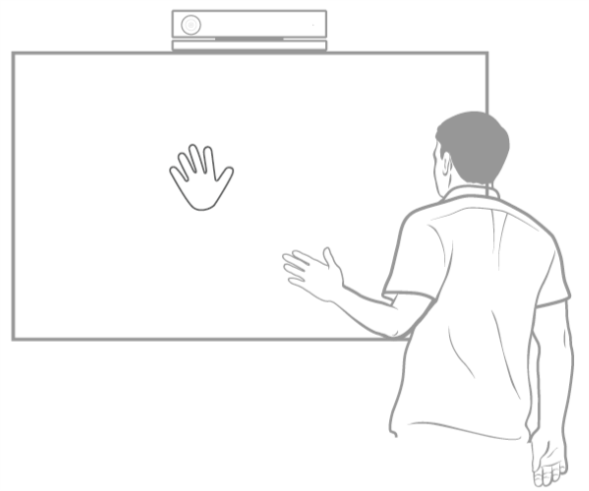
\includegraphics[width=0.5\linewidth]{Pictures/hciGuidelinesFeedbackCursor}
		\subcaption{Hand cursor}
		\label{fig:hciGuidelinesFeedbackCursor}
	\end{minipage}
	\hfill
	\begin{minipage}[t]{0.45\linewidth}
		\centering
		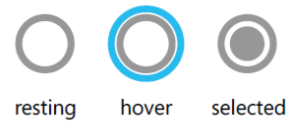
\includegraphics[width=0.5\linewidth]{Pictures/hciGuidelinesFeedbackControl}
		\subcaption{UI controls}
		\label{fig:hciGuidelinesFeedbackControl}
	\end{minipage}
	\caption{Feedback methods~\cite{MicrosoftHIG2014-mh}}
	\label{fig:hciGuidelinesFeedback}
\end{figure}

The most important part is the progress indicator described in this guideline. It says that an indicator should be given if the user has to hold a position, as well as the frequency of gesture repetition. Clear and prominent visuals should be used to show the entire progression (Figure \ref{fig:hciGuidelinesProgressIndicator}). If a user should copy a specific movement an avatar or animation can be shown, before or during the movement.

\begin{figure}[htb]
	\centering
	\begin{minipage}[t]{1\linewidth}
		\centering
		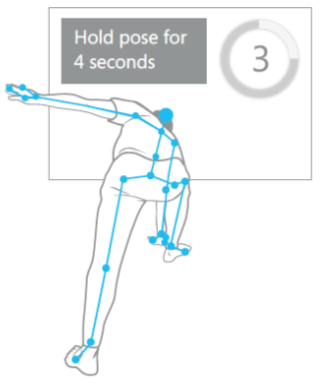
\includegraphics[width=0.27\linewidth]{Pictures/hciGuidelinesProgressIndicator}
		\caption{Repetition and time length indicators~\cite{MicrosoftHIG2014-mh}}
		\label{fig:hciGuidelinesProgressIndicator}
	\end{minipage}
\end{figure}


Summarizing the user interface should not distract the slacker but support him. Only necessary and useful information have to be displayed during the exercise. Providing an introduction and useful tips can help to give an understanding of the exercise. An avatar or animation is a good alternative to make clear how to perform an exercise. The system should also rely on Microsoft human interface guidelines, which provides design tips and serves as a reference to build user friendly applications.

%Kann evtl nicht genutzt werden
%Displaying an avatar can be further implemented by a conjunction or overlapping with an instructor on the screen \textbf{(Figure 8)}. With this she can see wrong performance execution in real time. After the exercise she should be able to review her performance. At the same time the system has to be aware of not distracting the user too much during the performance. 
\newpage

\section{Conclusion}
With the stated related work a foundation is given to build a slacklining assistance system. For teaching beginners on a slackline it is important get familiar with it. The assistance system should provide the given exercises and tips for beginners which build a foundation for further training.
%like focusing the eye and turning the hands over the shoulder, 
Several application scenarios show that slacklining can replace balance training in rehabilitation environment, as prevention system, in school sport or as an home assistance. This can be combined with interactive technology, which helps patients to fulfil their exercises and provide the medical stuff with sufficient analysis data.

As interaction device the Microsoft Kinect v2 seems like the best choice out of the available technologies. It provides sufficient useful and accurate data analysis, if no in-depth analysis is needed. More advantages are the low cost, short setup time and the freedom of the movements for the user. Several studies indicate also that the Kinect can be embedded in balance training scenarios and increases the training efficacy while motivate patients.

A problem that occurs with more complexity in the exercises is the raising cognitive load. The system should therefore provide appropriate feedback and be aware of the cognitive load of the slacker. Motivating the slacker for further exercise execution can be done with a well defined interaction mechanism, an enjoyable but challenging virtual training environment, and an user friendly interface. This can be realised especially with the help of human interface guidelines provided by Microsoft, which include several design tips for developing a Kinect application.

With the help of this foundation a concept for the slacklining assistance system has been created, which can be seen in the next chapter.
\newpage

\chapter{Slacklining  and Slacklining Learning Techniques}\label{3_slacklining}
The following section \textit{\nameref{3_1_introductionSlacklining}} gives an understanding of the evolution, philosophy, and basics of this sport. Further an overview about the diversity of slacklining and application scenarios can be found in section \textit{\nameref{3_2_slacklineVariations}}. The last section \textit{\nameref{3_3_learningTechniques}} elaborates teaching methods and exercises, which will be used as a basis for designing the concept and will be integrated into the system.
 \section{Introduction into slacklining}\label{3_1_introductionSlacklining}
The term slackline has its origin in the 1980's. Some climbers balanced on a tubular webbing in contrast to the existing balance activity tightrope, where you balance on a steel rope. Therefore they used the term \textit{slack wire} that later transformed into \textit{Slackline}, which means loose line~\cite{Zak2011-sl, Balcom2005-wl, MillerMauser2013-sl}.

Hence slacklining comes from the climbing sport and in a broader sense it can be compared with ropedancing~\cite{Kleindl2011-bl}. The line itself is made out of a nylon ribbon. Unlike in ropedancing the ribbons width is between 2.5 and 5 cm and is very flat. To fixate the line two stable fixation points are needed. Mostly it is then tensed between these points with a tension device, which is normally a part of the slackline. ~\cite{Kleindl2011-bl}. Because of the nylon texture the line will expand under pressure, if someone stands on it. Therefore it is very dynamic and the person has to outbalance every sway~\cite{Kroiss2007-ab}. Given this elasticity a person can e.g. bounce, bob, or swing on the line with which many application scenarios has resulted~\cite{Balcom2005-wl}.

\todo{phylosophy evtl erläutern}

 \section{Slacklining variations and categorization}\label{3_2_slacklineVariations}
Further depending on the length, tension or height a few slackline variations have originated~\cite{MillerMauser2013-sl, Kleindl2011-bl, Thomann2017-ab}. Regarding the height one can differentiate between a \textit{lowline} and a \textit{highline} (Figure \ref{fig:lowAndHighline}). The former is the category in which almost all lines match because it describes a height in which one can safely jump off the line. On a \textit{highline} this is not possible. Here you have to make safety provisions like a seperate system where the person can hook herself in this system above or under the regular line~\cite{Kleindl2011-bl}.
\begin{figure}[htb]
	\centering
	\begin{minipage}[t]{0.44\linewidth}
		\centering
		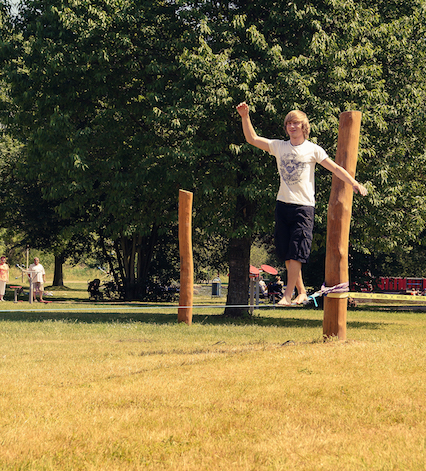
\includegraphics[width=0.94\linewidth]{Pictures/3_1_lowline}
		\subcaption{Common lowline}
		\label{fig:lowline}
	\end{minipage}
	\hfill
	\begin{minipage}[t]{0.44\linewidth}
		\centering
		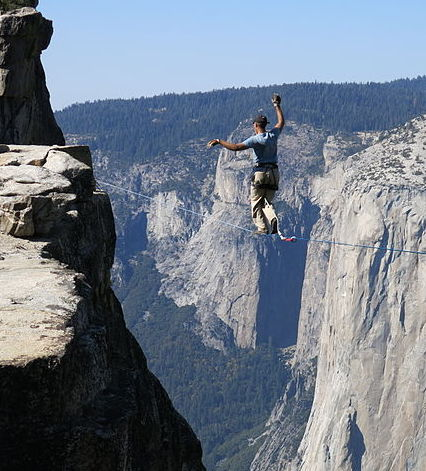
\includegraphics[width=0.94\linewidth]{Pictures/3_1_highline2}
		\subcaption{Highline between mountains~\cite{WikiSlacklining2017-lowline}}
		\label{fig:highline}
	\end{minipage}
	\caption{Low- and Highline}
	\label{fig:lowAndHighline}
\end{figure}

The following terms describe some fine granular variations of the slackline as well as categorizations in different application scenarios. They are not strict which means, they can differ in its scenario or \todo{blend/fade/merge} into each other. The \textit{trickline} (Figure \ref{fig:trickline}) is the common slackline. It is tensed a bit loose in about the height of the knees and has a length up to 30 m. A \textit{jumpline} (Figure \ref{fig:jumpline}) is stronger tensed to make jumps on the line possible. They have a length of 8 - 14 m and are a bit higher than the trickline. 

With a \textit{rodeoline} the line is actually more slacked and and has the highest amplitude, like seen in figure \ref{fig:rodeoline}. It is a relatively short line with a length of 5 - 8 m and the fixation points are in about 2 m such that if a person stands in the mid of the line it is just about above the ground and can swing on it. Slacklines beyond 30 m are called \textit{longline} (Figure \ref{fig:longline}). The goal here is to walk as far as possible without falling off the line. Beside these there exist some terms that describe a categorization or environment where a slackline can be applied. For example a \textit{waterlines} is simply a line tensed over a pool, sea or a river like in figure \ref{fig:waterline}. \textit{Urbanlining} can be found in urban areas, where manmade buildings or structures are used to tense the line between, like in figure \ref{fig:urbanline}.
\begin{figure}[htb]
	\centering
	\begin{minipage}[t]{0.45\linewidth}
		\centering
		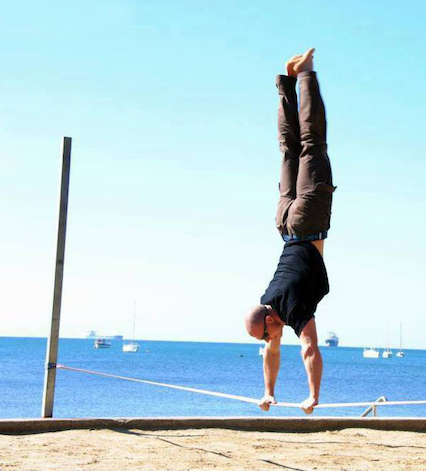
\includegraphics[width=1\linewidth]{Pictures/3_1_trickline}
		\subcaption{Handstand on a trickline~\cite{WikiSlacklining2017-trickline}}
		\label{fig:trickline}
	\end{minipage}
	\hfill
	\begin{minipage}[t]{0.45\linewidth}
		\centering
		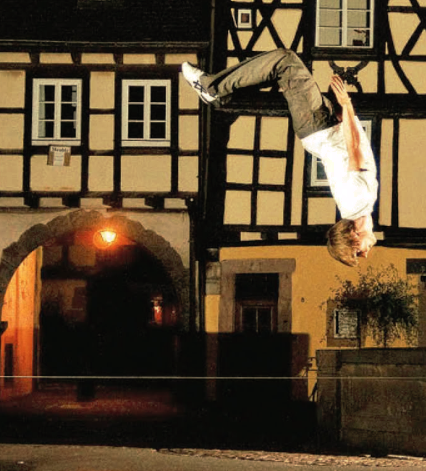
\includegraphics[width=1\linewidth]{Pictures/3_1_jumpline}
		\subcaption{Backflip on a jumpline~\cite{Kleindl2011-bl}}
		\label{fig:jumpline}
	\end{minipage}
	\hfill
	\begin{minipage}[t]{0.45\linewidth}
		\centering
		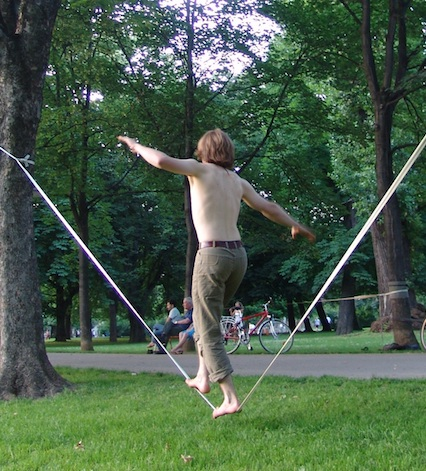
\includegraphics[width=1\linewidth]{Pictures/3_1_rodeoline}
		\subcaption{Rodeoline~\cite{WikiSlacklining2017-rodeoline}}
		\label{fig:rodeoline}
	\end{minipage}
	\hfill
	\begin{minipage}[t]{0.45\linewidth}
		\centering
		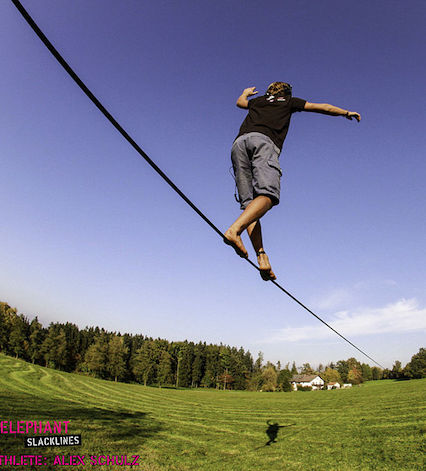
\includegraphics[width=1\linewidth]{Pictures/3_1_longline1}
		\subcaption{Longline~\cite{WikiSlacklining2017-longline}}
		\label{fig:longline}
	\end{minipage}
	\caption{Slackline variations}
	\label{fig:slacklineVariation}
\end{figure}
\clearpage
\begin{figure}[htb]
	\centering
	\begin{minipage}[t]{0.45\linewidth}
		\centering
		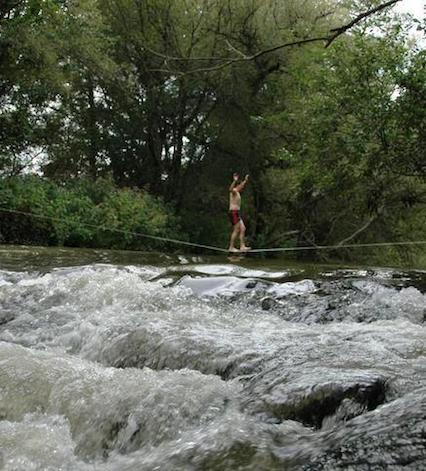
\includegraphics[width=1\linewidth]{Pictures/3_1_waterline}
		\subcaption{Waterlining over a river~\cite{WikiSlacklining2017-waterline}}
		\label{fig:waterline}
	\end{minipage}
	\hfill
	\begin{minipage}[t]{0.45\linewidth}
		\centering
		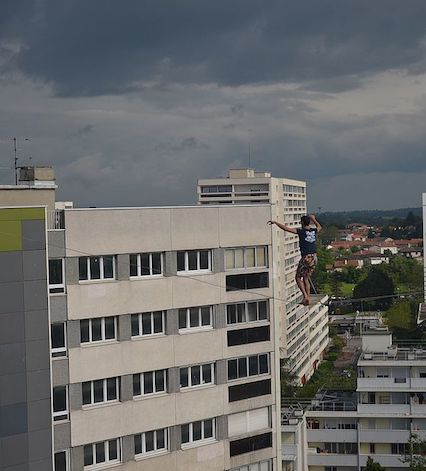
\includegraphics[width=1\linewidth]{Pictures/3_1_urbanline}
		\subcaption{Urbanlining in the city~\cite{WikiSlacklining2017-urbanline}}
		\label{fig:urbanline}
	\end{minipage}
	\caption{Categorization of slacklining}
	\label{fig:slacklineCategorization}
\end{figure}


 
 \section{Slackline learning techniques}\label{3_3_learningTechniques}
Section \textit{\nameref{2_1_1_slacklineTraining}} showed that systematic help is not essentially necessary to learn slacklining. The user of the interactive learning system should therefore be able to learn it by herself without any further external help. Therefore section \textit{\nameref{3_3_1_learningConcepts}} differentiates between two learning concepts on which the interactive learning system relies.
%Two learning concepts will be differentiated in subsection \textit{\nameref{3_3_1_learningConcepts}} to achieve this.
Further section \textit{\nameref{3_3_2_StagesExercises}} describes the categorization of specific slackline exercises in the system, which structures at the same time the learning flow of the user.

\subsection{Methods for slackline skill acquisition}\label{3_3_1_learningConcepts}
\subsubsection{Methodical routine}
A methodical routine can be integrated in almost every sport activity. It consists of a series of exercises, whose difficulty increases with further practice. The selected exercises should base on methodical principals that can be scaled by e.g. easy to difficult, known to unknown, or simple to complex~\cite{Fetz1996-ml}. Größing~\cite{Groessing1997-sp} describes the general procedure as follows: at the beginning of a methodical routine the trainee will perform warm up exercises. This is useful to prepare her for the training. After that preliminary exercise will be provided, which are more specific regarding the actual exercises. With this she will learn the general motoric basics and train the movements needed to perform the activity. Further it ensures a smooth transition for the main exercises.

Thomann~\cite{Thomann2013-aa} designed a methodical routine as well as a dynamical methodic for slacklining skill acquisition. His methodical routine inherits various approaches with different elements to reach the goal of learning slacklining. However the integration of these elements are more strict to guide the trainee through a constructive exercise procedure (Figure~\ref{fig:3_3_1_methodicalRoutine}). At first an introduction and preliminary exercises can be integrated. This follows by material and security where the lines dynamic, how to jump off, and controlling of the line is covered. Further the learning of the oscillation behaviour should be implemented with or without methodical help. Afterwards the user can decide to execute balance training with or without help. With help the trainee can directly balance on the line, which includes external support. Without any further help she can decide to first sit, step on the line, or balance independently. Continuing the trainee can decide if she wants to train the static or dynamic balance, which follows by the possibility for more variable exercise execution like walking forwards on the line, walking backwards, with eye closed, etc. Before going to train some tricks on the line, which is on the very end of the routine, the trainee has to learn first staying across the line with her feet. This is a necessary part for several tricks and has to be learned before.
\begin{figure}[htb]
	\centering
	\begin{minipage}[t]{1\linewidth}
		\centering
		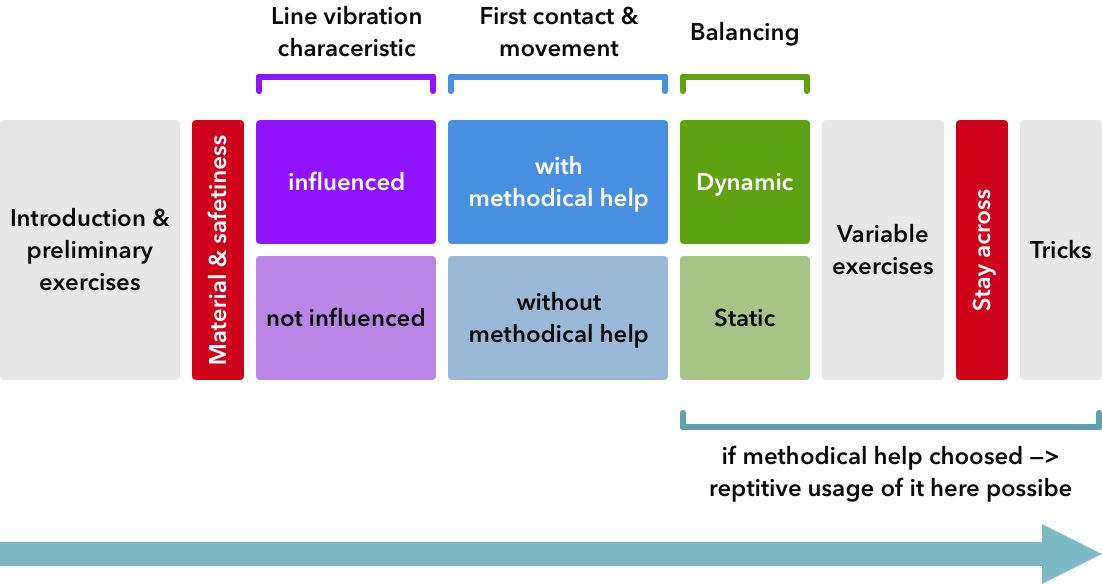
\includegraphics[width=1\linewidth]{Pictures/3_3_1_methodicalRoutine3}
		\caption{Methodical routine~\cite{Thomann2013-aa}}
		\label{fig:3_3_1_methodicalRoutine}
	\end{minipage}
\end{figure}

\subsubsection{Differential methodic}
The differential or dynamic methodic follows another approach. It is in coherence with an open learning situation~\cite{Thomann2013-aa}. This means it depends on several factors, which in slacklining would be line type and length, tension, environment, etc. Considering the interplay of these factors each trainee can construct her own training set. A dynamic methodic is a practical usage for this~\cite{Beck2008-dl, Schoellhorn1999-ip}. This inherits the model of stepping stones. In general it describes that many possibilities can lead to the same goal. Each potential way has therefore its own difficulty level. This results in a more modular way to reach a specific goal. In comparison to the methodical routine it results in bigger differences in stimulus and provide more variability in the movement execution, like compared in figure~\ref{fig:3_3_1_comparisonMethods}. 

\begin{figure}[htb]
	\centering
	\begin{minipage}[t]{1\linewidth}
		\centering
		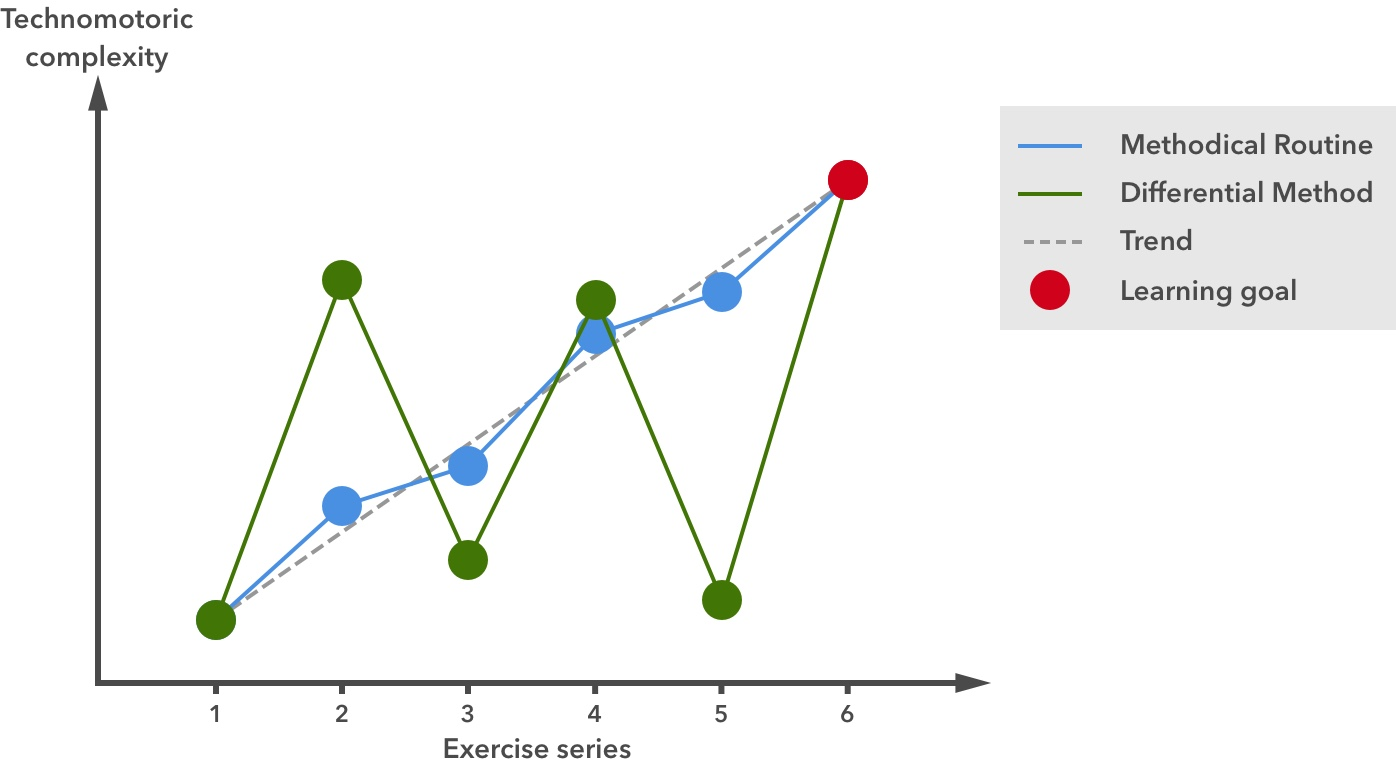
\includegraphics[width=0.83\linewidth]{Pictures/3_3_1_comparisonMethod2}
		\caption{Comparison methodical routine vs. differential method~\cite{Thomann2013-aa}}
		\label{fig:3_3_1_comparisonMethods}
	\end{minipage}
\end{figure}
To make us of the principle of differential learning the trainee can follow a methodical principle like seen in methodical routine. If she reaches a certain threshold of skill level more dynamic procedures can then be involved in the actual learn process. %Therefore the principle of differential learning can be used, which results in big stimulus differences and provide more variability in the movement execution.

The usage in slacklining can be integrated like described and visualized by Thomann~\cite{Thomann2013-aa} (Figure \ref{fig:3_3_1_dynamicMethod}). He divided exercises into five learning stages an in its coordinative demand and complexity. The main goal is to master controlled and complex movements on the line. The trainee has to choose an amount of various exercise of all stages. Each more complex exercise can either be supported by methodical help or the trainee can return to the lower stage to learn the movement for the specific exercise. Each trainee can therefore create her individual path. Modification and integration of more useful exercises are allowed. A structured examples can be seen in figure~\ref{fig:3_3_1_dynamicMethod}. The purple arrows visualize a way for people that are more coordinative, more venturesome, or have background knowledge. In contrast the green arrows visualize a path for people that are less coordinate, less venturesome, or have no background knowledge in slacklining.
\begin{figure}[htb]
	\centering
	\begin{minipage}[t]{1\linewidth}
		\centering
		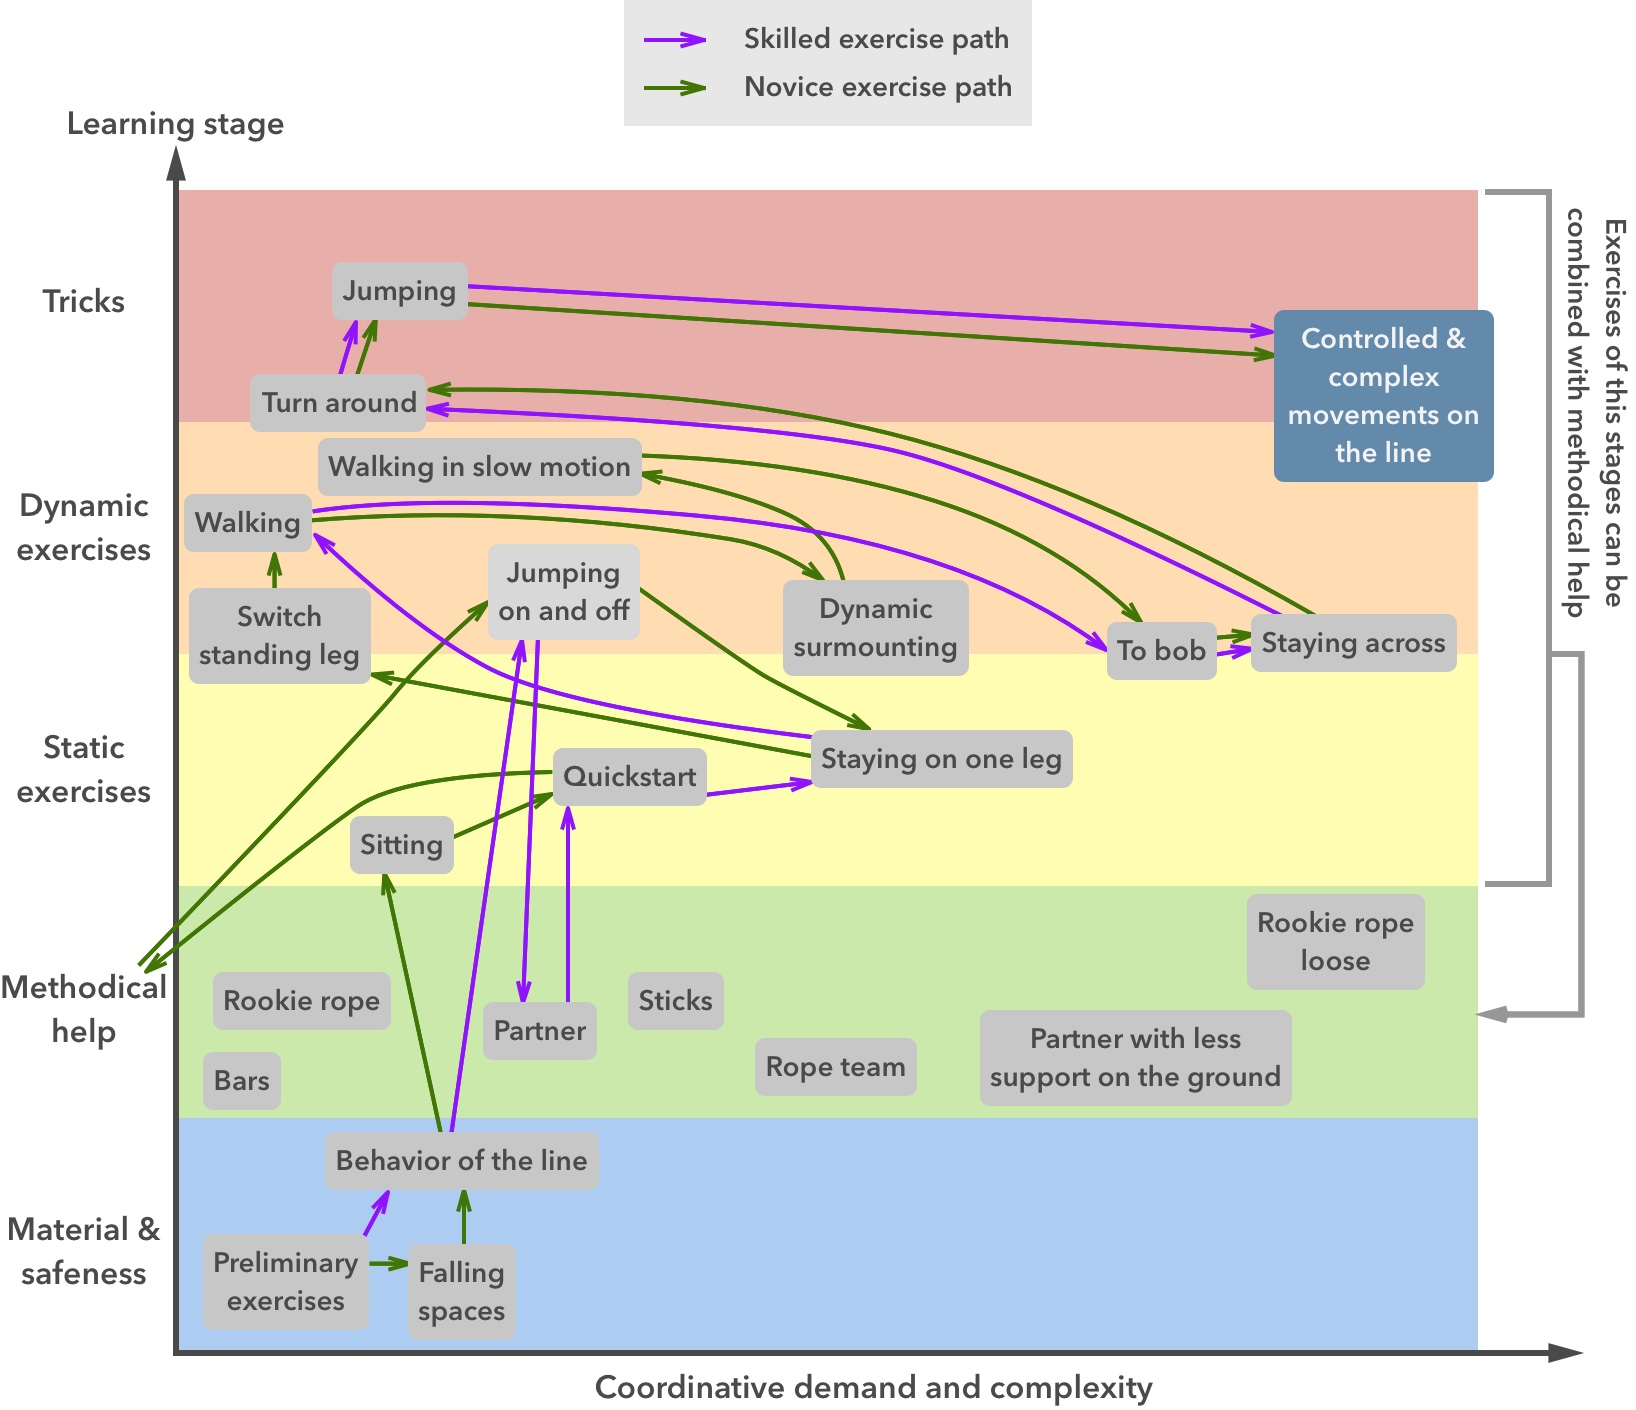
\includegraphics[width=1\linewidth]{Pictures/3_3_1_dynamicMethodBoth2}
		\caption{Dynamic methodic in slacklining~\cite{Thomann2013-aa}}
		\label{fig:3_3_1_dynamicMethod}
	\end{minipage}
\end{figure}

For proper user training with the system the trainee should follow a clear workflow. Therefore the methodical routine is the better choice as a learning concept in this interactive learning system. She learns right from the beginning essential aspects of slacklining that are relevant and build up on each other. Because it follows a strict linear sequence stages and exercises can be designed as levels. 
%The trainee can unlock further levels by successfully executing the prior exercise. 
The next subsection \textit{\nameref{3_3_2_StagesExercises}} will therefore cover a clear workflow integration of exercises for this learning system.

\subsection{Stages and exercises of learning slacklining}\label{3_3_2_StagesExercises}
% Drei verschiedene Grundfertigkeiten: zunächst muss man auf einem Bein stehen können, dazu kommt die schmale Unterstützungsfläche, auf der man balancieren soll. Nicht zuletzt befindet man sich in einer gewissen Höhe und nicht mehr auf sicherem Boden.
Now that an overview about slacklining and its learning techniques are given several practical exercises have to be considered. Repetitive trials are one approach of learning to walk on the line. However this could result in dangerous situations and frustration of the slacker because of her missing skills. Therefore an exercise set is elaborated that teach and guide the slacker. The teaching goal should be that the slacker can balance with a controlled manner on the line, stay on it for a few seconds, and be able to walk a few steps. In general one has to acquire three core skills to achieve this goal~\cite{Kroiss2007-ab}. At first the slacker should be able to stay on one foot. This is essential because most of the time the slacker has a standing foot on the line and the other one servers as balance component. Second the balancing on a narrow surface since the slackline exists of a limited width. Lastly managing the height is also important due to the fact that the slackline is mostly tensed around the knee height and above.

As a groundwork the elaborated exercises are based on Kroiß~\cite{Kroiss2007-ab}. He elicited learning exercises for beginners on a slackline within a school class, which gives a good basic on the exercise integration. Further several other references~\cite{Balcom2005-wl, Donath2013-kk, Donath2016-gm, Granacher2010-ow, Keller2012-xh, Kleindl2011-bl, Pfusterschmied2013-yy, Thomann2013-aa} have been researched to elaborate exercises that fit the best in this system. Each exercise is therefore categorized in one of four tiers, which represent the fundamental basis of the exercises routine. In the following each tier is introduced, its goal clarified, and the learning aspects described:

\subsubsection{Tier I - Preliminary exercises}
The first tier serves as a preparation for the subsequent exercises. Hence just exercises on the ground will be executed. This is to train and strengthen the persons general physical balance. In general it is recommended to train barefoot or with socks to get a better foot feeling. The knees should be bent to have a better initial position for movement compensation. Keeping the head up and setting a focus point can help to calm the visual sense of balance. In almost all exercises of this tier the arms have to be stretched to the side, be over the shoulder, and bent in about 135 degree. This is the biggest balance function overall because you have freedom in all directions and the slacker can shift her body's center of gravity. Further all exercises should be executed slowly and controlled to master the body behaviour.

\subsubsection{Tier II - First contact with the line}
Mastering the general physical balancing leads the slacker to her first experience with the slackline. The goal is to get a feeling for the slackline and to be able to get up on the line as well as hold herself for a short amount of time. For this the slacker has to become familiar with the line, feel the imbalance, how her body wants to behave, and get a feeling for counterbalancing unpredictable movements. Therefore starting at the sweet spot, that's about 1/3 of the line, can help. It's an area with a comfortable vibration characteristic. The foot should also be always in alignment with the slackline to have the biggest amount of surface of your foot covered with the line, which results in more contact area of the foot. If the slacker has problems with holding her hands over the shoulder, she can turn the palms to the top and the hands will then raise automatically up. A relaxed but straight upper body can help to hold the right position.

\subsubsection{Tier III - Static exercises}
More difficult exercises come in this tier. The slacker is now familiar with the line and able to stand for a short amount of time on it. The goal is that the slacker should stay confidently on the line. Further it serves as preparation for walking on the line. All prior learned techniques have to be directly applied. The non standing leg now comes more into action. It serves as an additional balancing parameter to both of the arms. If the slacker has problems with going up on the line, she can keep the balancing leg vertically in line with the standing leg while going up and then move it to the side. The pressure is mostly around the ball of the foot.

\subsubsection{Tier IV - Dynamic exercises}
This is the last tier and it involves the dynamical part for the slackline. The slacker should now be able to stay confidently on the line with one foot and both feet. The goal is to learn how to make the first steps as a result for walking on the line. In general it is applying static exercises together. While staying on the line and when the slacker wants to make a step she can guide her balancing foot to the side of the line and shift it then forwards. Letting the knees together when making a step forward helps because the legs can support each other. Making small steps won't shift the body's center of gravity that much forward, which results in more control.

 
 \section{Conclusion}
Slacklining can be compared with ropedancing but with a wider and flater ribbon. It is a sport that claims a certain amount of balancing skills. Therefore, two learning techniques have been discussed for skill acquisition, which are the methodical routine and dynamic method. The interactive learning system presented in this work will focus on the methodical routine. This technique follows a clear workflow and its structured routine can be easily implemented into the system as a prototype. With the help of Kroiß~\cite{Kroiss2007-ab} and other works a set of exercises have been designed that fit in this routine and train beginners appropriately.

  
\chapter{Concept}\label{4_concept}
This chapter describes the conceptual analysis of an interactive slackline learning system (SLS) with real-time feedback. The idea of the SLS is to provide helpful information, structured exercises, and appropriate feedback to the user for learning slacklining with the given application. 
%One main feature is the autonomous interaction with the system. 
The user should be able to interact independently of any controlling device or external support like human help. Therefore, the SLS can only be controlled by the currently interacting user. Further, it responds appropriately to the actions of the user and provides several real-time feedback indicators to support her during the exercise execution. 

In the following conceptual analysis will be elaborated. Section \textit{\nameref{4_1_general}} describes basic design principles and system related requirements. This is followed by the more specific sections \textit{\nameref{4_2_interaction}}, \textit{\nameref{4_3_stages}}, and \textit{\nameref{4_4_exercises}} that describe how to interact with the system and how exercises are structured. Another main component is to provide adequate feedback to the user, which is part of section \textit{\nameref{4_5_feedbackSystem}}. Lastly section \textit{\nameref{4_6_scenario}} gives a good overview about the workflow of the specific components.
\section{General Information}\label{4_1_general}
In general the system should be easy to understand, to learn, and to interact. To achieve this it should provide proper user experience. Usability heuristics are useful to identify or to prevent problems in a system. Therefore the system will rely on the interaction design principles by Nielsen~\cite{Nielsen_1994-he} described in section \textit{\nameref{nielsenDesignPrinciples}}. Beside this certain tasks have to be considered that are more related to this system. An overview about these can be found in section \textit{\nameref{systemBasics}}.

\subsection{Ten heuristic principles for interaction design}\label{nielsenDesignPrinciples}
Nielsen designed his ten heuristics by comparing several sets of usability heuristics with existing usability problems from certain projects~\cite{Nielsen_1994-he}. Hence he was able to determine what heuristics identify usability problems the best and therefore creating a set of them. To prevent that a system results in having such problems they can also be used as a guideline for designing and developing a user friendly system. The interactive slackline system will follow these principles, which are described in the following:

\textbf{\hyperref[4_1_1_visibilitySystemStatus]{Visibility of system status}}\\
The system should always keep the user informed about the current state through appropriate feedback in an adequate time.\\

\textbf{Match between system and the real world}\\
The system should provide the user with familiar terms and information. Using technical terms with which she is not familiar can lead to confusion. Therefore proper information should be natural and in a meaningful order.\\

\textbf{User control and freedom}\\
If the user clicks accidently on something she should be able to leave this state without any troubles.\\

\textbf{Consistency and standards}\\
It should follow a clear design standard and provide consistency. The user should not be confused whether different terms or elements mean the same.\\

\textbf{Error prevention}\\
Conditions and actions that could easily result in errors should be prevented. Another option is to inform the user about the consequences that the action may have and which she has to actively confirm.\\

\textbf{Recognition rather than recall}\\
The users memory load has to be minimized. She should not remember every action or information. Elements, actions, and options should be visible and instructions about the usage must be easy to retrieve.\\

\textbf{Flexibility and efficiency of use}\\
Providing quick options and allowing to skip certain steps can speed up the interaction for more familiar users. Hence the system should take care of both novice and experienced users.\\

\textbf{Aesthetic and minimalistic design}\\
Information should just contain aspects that are relevant to the user and that she really needs. Every irrelevant data decreases the intelligibility.\\

\textbf{Help users recognize, diagnose, and recover from errors}\\
Error messages should accurately indicate the ongoing problem such that the user knows what is wrong. Providing a constructive solution helps the user to solve the problem.\\

\textbf{Help and documentation}\\
Optimally the system can be used without any further documentation. It may be the case to provide help and documentation. If it cannot be circumvented it should be easy to find it and clearly show the relevant steps.\\

\subsection{System specific basics}\label{systemBasics}
One person at a time should be able to interact with the system. This is because mostly just one person can stay on the slackline especially for beginners. However it should provide the ability to have multiple user profiles. One can switch between those such that several persons can have a profile on the same application. For proper user training the system should follow a clear workflow. Therefore two methods have been discussed in section \textit{\nameref{3_3_1_learningConcepts}}. A methodical routine will be used with which stages and exercises can be designed as levels. These should be locked at the beginning and the user can unlock them by successfully executing the prior exercise. Another important part is the user tracking. The system should be able to track the user in an appropriate accuracy and precision such that it can match the users movement with the actual exercise. This is in correlation with properly providing real-time feedback, which is further discussed in section \textit{\nameref{4_5_feedbackSystem}}. All relevant recorded data should be immediately saved when it is needed, e.g. when successfully accomplishing an exercise.

\begin{comment}
- System should be able to track user appropriately
- All relevant data should be immediately saved when it is needed (unlocking exercise/stage, failing/accomplish exercise)
- Information about where the user currently is should be given --> title
- User selection
- Also a possibility to go to the last screen if she misclicks should be given.
\end{comment}
\section{Interaction}\label{4_2_interaction}
A bigger part of the system is the interaction since it is independent of any external controlling devices.
The user should be able to navigate through the system by herself with her hands as interaction input.
A cursor should always be visualized to navigate through the systems interface.
If the user initially starts the system, there should be an engagement gesture to convey that the system initially recognises and responds to a user action.
Furthermore, a small tutorial should be given in which the user will be trained on how to use the interaction possibilities with the system (\textit{cf. \hyperref[nielsenDesignPrinciples]{Recognition rather than recall}}).
To make her familiar with these, she should directly apply these techniques in the tutorial.
The current state of the interaction is clearly visualized, such that the user knows if she triggers an action regarding an element (\textit{cf .\hyperref[nielsenDesignPrinciples]{Visibility of system status}}).
To be able to interact with elements and start the exercise execution the user should stay in a predefined initial position.
The SLS then recognises if a user is ready to start. Interaction will also play a role in exercise execution.
During the execution she interacts with the SLS by trying to match the predefined exercise.
The user should then get appropriate feedback, which is further explained in section \textit{\nameref{4_5_feedbackSystem}}.

\begin{comment}
- user can and should interact with the system
\\- Cursor visualization as hand image
\\- Engagement gesture for first interaction with Kinect (One hand over shoulder)
\\- She should be instructed how to interact 
\\- Different interaction methods should be provided to prevent failing on one (tutorial --> clicking (variations) + scrolling)
\end{comment}
\section{Stages}\label{4_3_stages}
The system covers predefined gestures, which are subdivided in stages that have been elaborated in subsection \textit{\nameref{3_3_2_StagesExercises}}. Since the interactive slackline system follows a slightly exergame like approach, the stages and exercises should be designed as levels, which the user could select has to unlock. Therefore a menu should exist for all available stages as well as for all exercises within a stage. To give her a starting position, the very first stage and exercise should be interactable. 
She can then unlock the next stage by accomplishing all exercises in the last one. Hence it can be assured that the user is able to encounter with the more difficult exercises. She should also be introduce in each stage to know how its purpose and goal. At last a summary can be given to show an overview of her performance for the entire stage.

%The user should also be introduce in each exercise to know how to perform it correctly and give her support for successfully executing it

\section{Exercises}\label{4_4_exercises}
%should have predefined exercises that can be tracked in an appropriate manner
Each exercise is part of one stage. It is divided into two body sides, which consists of several repetitions (Figure \ref{fig:exerciseStructure}). Every exercise is locked except the first one to provide a starting point, like with the stages. The next exercise should be unlocked by accomplishing both sides of the current one. Similarly a side will be completed if all repetitions have been finished. Like for the stage, each exercise should be instructed for the user such that she can successfully perform it. The system will also recognise if the user is ready to start with the exercise. During the execution she should get real time feedback about her current performance. An exercise summary should then show the performance of the execution with several performance parameters regarding the given exercise.

\begin{figure}[htb]
	\centering
	\begin{minipage}[t]{1\linewidth}
		\centering
		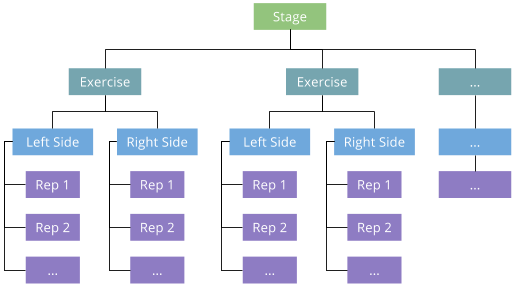
\includegraphics[width=1\linewidth]{Pictures/exerciseStructureTopDown2}
		\caption{Exercise structure}
		\label{fig:exerciseStructure}
	\end{minipage}
\end{figure}
\begin{comment}
\\- system should provide predefined exercises that can be tracked per user
\\- A stage menu should be provided to the user, which shows her the amount of stages to complete
\\- It consists of 4 stages each with specific exercises (Preliminary, First contact with slacklining,  Static exercises, Dynamic exercises) like explained in chapter 3
\\- A stage consists of several exercises like explained in prev. chapter
\\- locked stages (initial first stage interactable)
\\- unlock stages (by successfully accomplishing all exercises from current stage)
\\- Stage introduction gives general information, describes the goal and tips for the current stage
-- a stage information scene provides her with the general introduction of this stage --> unlocks first exercise
\\- Stage summary contains average data about each exercise
\end{comment}

\section{Feedback system}\label{4_5_feedbackSystem}
%The user should get feedback about her performance during exercise execution. 
%Another big role of this plays in the exercise execution. Here the user interacts with the system to match a predefined gesture for accomplishing the exercise. Therefore real time feedback is provided which gives her hints about the right interaction and how good it is performed. More information about the feedback methods can be found in feedback system

% - https://www.researchgate.net/profile/Eduardo_Velloso/publication/262162999_MotionMA_Motion_modelling_and_analysis_by_demonstration/links/577a4aaa08aece6c20fbc5bf.pdf
% - https://www.ncbi.nlm.nih.gov/pubmed/27555917
% - http://online.liebertpub.com/doi/abs/10.1089/g4h.2012.0041?url_ver=Z39.88-2003&rfr_id=ori%3Arid%3Acrossref.org&rfr_dat=cr_pub%3Dpubmed&
% - https://www.ncbi.nlm.nih.gov/pmc/articles/PMC4835340/
% - http://ieeexplore.ieee.org/document/7399879/

% - https://www.akqa.com/work/nike/kinect/
% - https://www.ea.com/de-de/news/ea-sports-active-2-bringt-fitnessfans-in-die-form-ihres-lebens

Feedback is the main and most powerful component of the interactive learning system. Since the user should interact on her own with the system one has to assume that no other person interfere with her and the system. With this in mind the feedback of the system should designed in a way, that the user knows at any time what she has to do or has done. In general audio and visual feedback will be provided to the user. Regarding the \textbf{\nameref{4_2_interaction}} with the system, e.g. clicking a button, the system should respond with an audio signal and change the elements visual state accordingly.

For the accomplishment of the exercise execution it is essential to provide real-time feedback. This supports her during the performance and enhances the learning effect more than with post feedback methods, like discussed in \textbf{\nameref{2_3_3_feedbackApproachesTechniques}}. Hence the overall exercise execution can be improved by providing appropriate real-time feedback. The system should therefore response to the user like seen in other applications \textbf{\todo{[cite, maybe Related Work --> Nike + / EA SPORTS Active 2]}}. These responses should mainly contain an indicator if the execution is currently performed right or not, visualize the the performance of the user regarding the predefined gestures, and the progress of the the current execution. The user should also see herself mirrored in an appropriate environment to know how the executes the exercises and if she is in detection range of the kinect sensor. With this a baseline is built for appropriate real time feedback to the user.

\begin{comment}
- in general audio and visual feedback
- if the user has clicked a button
- stays in the right position
- Indicator about if exercise is correctly executed
- Indicator about how good the exercise is performed
- real time feedback (Time, confidence, checklist, repetitions)
- system should inform how many repetitions are left
- system should inform when the repetition is successfully accomplished (audio, visual -> timer green, repetition counter)
- system should inform the user if repetition was not successful (audio, visual -> reset timer, checklist)
- After successful execution, a summary is shown about the performance of the user for each rep (time, attempts, confidence)
- tier summary (avg. time, attempts, confidence)
\end{comment}

%\section{Scenario}\label{4_6_scenario}
%To have a better understanding regarding the interplay of the several components a generic scenario workflow will be given from a users' point of view. The users' name is Bob and he is 21 years old. While climbing with friends in a climbing hall he noticed a new interactive learning system that they provide to visitors for trying and learning slacklining. He heard once of this activity by friends but never had the chance to try it. So he decides to test it and wants to execute some exercises. To engage with the system he has to stay in front of it, which recognizes him immediately. At the beginning it introduces him regarding the interaction possibilities. After that, he selects a tier and is further informed about the goal and basics of this stage. Once confirming that he read everything it leads him to the first available exercise. The system shows him how to execute it properly. Right after starting the exercise he gets helpful real time feedback to correct himself for a successful accomplishment of the execution. After finishing the exercise Bob gets an overview about his performance.

%asks him to do an engagement gesture. Now he is introduced in the interaction of the system. After he knows how to interact with the system he can select a user profile, which was created by the personal before. This will lead him to the stage selection. He selects the very first because all others are locked. In here bob has to read the instructions for the stage to be informed about what he has to pay attention for. Next he selects the first exercise and a body side he wants to train. Before bob can start with the execution, he will be informed about how this specific exercise is executed and how to perform it. After he thinks that he is ready to challenge it, he starts the exercise explicitly. Now he sees all relevant information about the execution and starts to execute it. He notices that the system gives him real time feedback about his performance and the progress made. After finishing all repetition the system leads him to the exercise summary screen, which gives an overview about the performance of the just executed exercise. 

%The user raises the hands over her head to start the application. She is now instructed on how to interact with elements on  the screen, e.g. clicking and scrolling. After being confident with this, she selects her user profile to load the appropriate exercises and leads her to the stage selection. She selects the first stage since all others are currently locked. Now she is in the exercise menu. In here she clicks on the \textit{stage information} button, which gives her an introduction into the stage. After confirming that she has read the introduction the first exercise becomes unlocked and she selects it. After that she decides to train her left leg first in the side selection. An exercise introduction screen is following, which shows specific information about the execution. After reading the introduction she feels ready to counter the exercise. Therefore she goes into the starting position and starts the exercise by clicking the start button.

%The screen changes and all relevant elements are shown for the exercise execution. She performs every repetition of the exercise successfully. After finishing these the system leads her to the exercise summary screen, which shows her the performance of the just executed exercise. In here she can now decide to return to the main menu or go on and start the training for the other body side. This procedure is also visualized in Figure \ref{fig:scenarioWorkflow} below.

\section{Conclusion}\label{4_7_conclusion}
\chapter{System integration}\label{5_systemIntegration}

\section{Hardware}
- Kinect

- Beamer

- Screen

- Slackline --> Alpidex High Performance

\section{Software}
- KinectStudio

- VGB

- Unity3D

- Kinect SDK for unity

- Kinect MS-SDK

\section{User Interface}
Besides this she is instructed on how to stay in the right starting position. This is required by some actions like just before starting the exercise execution to ensure the user is ready.

The user should be introduced to the stage. In here the purpose, goal, and helpful techniques should be given, such that the user becomes an overview about the exercises. At last a summary scene shows several performance parameter for the exercises in this stage.

She should stand in a starting position to start the exercise. This is to ensure that no exercise is starting to track if the user would make a random gesture which could lead to confusion of the user.
\subsection{Cursor}
Specifically for the cursor, with which the user can interact with elements on the system by pushing the hand towards the kinect, the state will be clarified by a circle like seen in figure \todo{insert figure below}.

The state of the current interaction is visualized properly by providing a circle around the hand cursor that represents the progress like seen in figure \ref{fig:handcursorProgress}.
\begin{figure}[htb]
	\centering
	\begin{minipage}[t]{1\linewidth}
		\centering
		
\includegraphics[width=0.6\linewidth]{Pictures/handcursorProgress}
		\caption{Progress of handcursor (Left: Default, Middle: In progress, Right: Finished)}
		\label{fig:handcursorProgress}
	\end{minipage}
\end{figure}



The user starts with an engagement gesture like raising her hand over the head to convey that the system initially recognises and responds to a user action. After that a tutorial about the interaction with the system will be given that covers clicking and scrolling techniques. Now she's confident with the system interaction and can select a profile in the user select to train. This loads the profile which leads to the stage selection menu. In here she can select a stage, whereas initially the first one is can be selected and the others have to be unlocked by successfully accomplishing all exercises in the preview stage. Selecting a stage leads to the exercise menu. In here she has to read initially the stage introduction to become a basic understanding about the exercises in here. After reading this, it unlocks the first exercise. Selecting an exercise leads to the side selection, where the user has to choose the side she wants to train for this exercise. This is followed by an introduction of the exercise, in which is explained how to perform it correctly. If the user is ready, she should stay in a starting position to be able to start the exercise execution. In here she find all relevant elements to perform the exercise, like indicators for the time, repetitions, confidence and a checklist, which helps her to correctly execute the exercise. After successfully executing the exercise, a summary is shown which summarizes the user performance. Then she can return to the main menu or directly approach the next exercise. A stage summary gives an overview about all exercises with average performance parameters.

\todo{replace figure with directional flow}
\begin{figure}[htb]
	\centering
	\begin{minipage}[t]{1\linewidth}
		\centering
		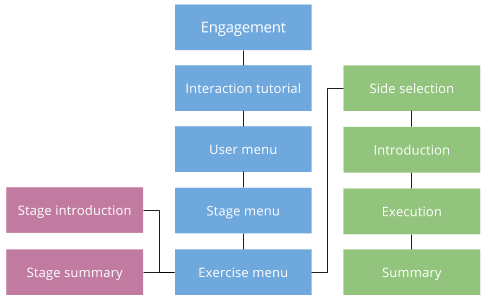
\includegraphics[width=0.8\linewidth]{Pictures/conceptScenarioFlow2}
		\caption{Scenario workflow}
		\label{fig:scenarioWorkflow}
	\end{minipage}
\end{figure}

\section{Real time feedback}

 In the slackline system the following feedback indicators are integrated for the exercise execution:
\begin{itemize}
\item Staying in the right position before starting an exercise
\item When an exercise is currently correctly performed
\item How good the exercise is currently performed, namely the confidence
\item The elapsed time the user is performing the exercise
\item When the repetition is successfully accomplished, i.e. the minimum time has been reached
\item When an repetition attempt was not successful
\item How many repetitions in general, finished and left
\item Checklist about key elements in an execution (like hands up, foot stretched, etc.)
\item A summary that shows the user parameters about the performance (execution time, overall attempts, confidence) for each repetition and an average value of these
\item A similar summary can also be found for the entire stage, where the same parameters for each exercise are listed in average
\end{itemize}

\section{Proof Of Concept}\label{3_3_proofOfConcept}

A few questions have to be clarified before starting with a concept of the assistance system. First if it is possible to track a human body on the slackline with the Kinect v2. Is the answer positive than the second question should be how good is the tracking behaviour of the device and can it therefore be used to track a human body on a slackline.

\subsection{Introduction}
As seen in several movement scenarios, in the area of balance training, the user were successfully trackable by the appropriate device \textbf{\todo{[CITE]}}. Hence the expectation is that the Microsoft Kinect v2 should be able to track the human body on a slackline with an appropriate accuracy and precision. But the range of the slackline, the movement of the line itself, unpredictable movements of the user, and his balancing actions could also possibly disturb the tracking ability. This can then lead to imprecise and inaccurate tracking data that negate the stated findings of other tracking balancing scenarios.

With this in mind multiple angles, positions of the camera, as well as the slackline have been tested. This Chapter will therefore describe a feasibility study, which gives clarification about the named questions. 

\subsection{General setup of the study} %Mobile slackline device and constraints with the Kinect v2 vamera view
One essential part that is needed for the experiment is the slackline. But it exists in many different forms and variations as seen in the \textbf{\nameref{3_1_introductionSlacklining}}. Also all lines have to use a fixing mechanism and are normally attached on a tree, pole, pillar, or with anchors on the ground or on a wall. In the case of this study, it would result in a constraint of variability. 
The choice felt therefore on a mobile slackline device variation, which is the most suited alternative. It consists of a slackline itself that is tensed around brackets at both ends. For feasibility reasons and because the focus of this scenario lies mainly on beginners, the device is comparatively short. A variable middle rail can be telescoped and vary the length of the device from \textbf{\todo{1 m up to 3.5 m}}. With this it is possible to test it indoors and in different positions with a minimum of effort \textbf{ \todo{figure x}}. Another advantage of this is the independence and variability of the device. This makes it easy to test it for the best position regarding the tracking camera, which is another essential part of the experiment.

In slacklining the user should be free in his movement and match predefined gestures. Therefore the low-cost tracking camera Kinect v2 is used as tracking device. As discussed in \textbf{\nameref{2_3_interactiveTechnology}} this is the most appropriate one out of the available user tracking devices.
A mentionable role plays the detection range of Kinect’s depth sensor regarding the length of the slackline. The sensors range lies between \textbf{\todo{0.5 up to 4.5 meters [CITE]}}. Since a mobile slackline is used with a length up to 3.5 meters, it would fit entirely in the tracking range. To track user for further training on a longer slackline, the depth range is not sufficient. This could be solved by using more than one Kinect device to have a larger the range. 

Generally a major point for tracking the user is the interplay between positioning the tracking device and slackline The coherence of angle and height of the Kinect v2 is essential for the depth range, which varies by changing these parameters. This will be discussed in the following.

\subsection{Testing scenario}

The study took place in the laboratory of the research group in the \textit{\textbf{german reasearch center for artificial intelligence}}. A big advantage of this is the large space to place the slackline in different variations. The slackline can therefore be easily moved and is faced in three positions to the Kinect - frontal (0 Degree), diagonal (45 Degree) and sideways (90 Degree) \textbf{\todo{(Figure X)}}. Each of this positions is tested regarding three different height level of the Kinect v2. Therefore it is attached on a tripod like seen in \textbf{\todo{Figure X}}. At the end nine different combinations are covered to track a user on a slackline, which gives a good coherence of the camera height position to the slackline direction. In the following the results discuss the feasibility of the coherence. With this a good overview is given to find appropriate tracking positions.

\subsubsection{Slackline positioning}
\textit{\textbf{Sideways}}


Here is the slackline positioned sideways, in 90 Degree rotated to the Kinect v2. The advantage of this is that the whole body on the slackline is in a constant line within the tracking area of the Kinect v2. With this no interference regarding the tracking distance can happen \textbf{\todo{(Figure X)}}. But the result show that regardless of the Kinect height the user tracking is very bad. This is because many body parts overlay and the Kinect v2 has problems to detect the body joints with appropriate accuracy and precision, which can be seen in \textbf{\todo{Figure X}}. Therefore this seems not like the appropriate slackline position.

\textit{\textbf{Diagonal}}

The slackline stays diagonal in 45 Degrees to the camera view. Because of this there is now a distance between front and end point of the slackline. This is not a problem because it fits well in the tracking range \textbf{\todo{(Table X and Figure X)}}. This could even result in a better trackability in matter of the depth field range, since the distance in the front shrinked and is therefore closer to the Kinect depth view. Another advantage is that many body party doesn't occlude entirely here because of the angle to the camera. Therefore a better tracking ability is given than positioning the slackline sideways.

But this problem is not entirely solved. It occurs with occluding joints of the slacker at the end of the line due to the angle the arms and the body \textbf{\todo{occlude/interfere}} with each other. Also the whole leg occludes the other one while stepping forwards \textbf{\todo{(Figure X)}}. This results in a not entirely perfect joint tracking and can lead to detection problems, depending on the executed exercise.

\textit{\textbf{Frontal}}

In the last positioning the slackline stays frontal in line with the user facing towards to the Kinect camera. The distance takes almost the whole range from the Kinect’s depth field up to the edge of it \textbf{\todo{(Table X)}}. The advantage is the user tracking ability which is here the best out of the three positioning. The camera can see the full body and have nearly no problems with occlusions.\\
One problem could occur with overlaying feets if the slacker stay with both feet on the line, which is in this case independent to the Kinect height \textbf{\todo{(Figure X)}}. But testings regarding this problem have not shown any critical detection problems. The Kinect can calculate the location of an occluded joint with a certain tolerance due to its own algorithms \textbf{\todo{[CITE]}}.

\subsubsection{Kinect height}
Three main height levels were used to show the main differences of the tracking behaviour from the Kinect. It is mounted on a tripod and covers the heights seen in \textbf{\todo{Table X}}, within the range of 0.80 meters up to 2.40 meters from the ground. 

Beginning with a height of 2.40 meters the Kinect has a very steep angle to track the slackers body on the full range of the slackline. Because of this the depth range shifts into the front like seen in \textbf{\todo{Figure X}}. Therefore if the slacker begins at the starting position on the slackline, he immediately reaches the end of the tracking area which can cause tracking problems. Because of this steep angle the joints will occlude other, the further he walks to the end of the line.

A step lower with a height of 1.60 meters the entire body is fully visible in almost all ranges. The Kinect is now on a level with the users shoulder and has therefore a relatively flat angle. Because of this the slackline has to be positioned a little bit further away as former to be fully visible for the Kinect view. This results in a more homogeneous depth range view like seen in \textbf{\todo{Figure X}}.

Problems can occur at the very end of the slackline depending on the slacker’s height. It could be the case that his head or more will be cropped. Therefore the slackline has to be slightly further away from the Kinect camera than on other heights. But for beginner training purposes this is not relevant.

A height of 0.8 m results in an even more flat ground perspective. The Kinect is now a little above the level as the slackline. Like in the last one the whole body is in the entire line good visible, but here also at the very start of the line. Problems can occur here with the tracking ability at the starting point. This is because the full tracking range is used \textbf{\todo{(Figure X)}}. Therefore at the very end  

Overall a range of 0.80 m up to 1.60 m seems like the best height for the Kinect for tracking a slacker. The tracking and view is more homogeneous and the angle is flatter with which the full depth range can be used.

\subsection{Best positioning for beginner learning purposes}
The frontal positioning has the only big problem with the depth range at the starting position of the slackline. Since only beginners are the main focus of this study, the starting position of the slackline plays an important role. Therefore for tracking purposes it is better to move the slackline closer to the camera. With this the last quarter of the slackline is cropped out of the view but the slacker can be tracked with a higher confidence \textbf{(Figure X)}. The Kinect height should be between 0.8 and 1.8 meters. With a higher attachment the angle will be too steep and the available space is cropped, or occlusion of body parts can occur.

\todo{\textbf{table}}
\chapter{Study}
%The interactive slackline system should be  in an \todo{explorative?} user study. 
%The elaboration, preparation, execution, measurement, and analysis is part of this chapter. 
This chapter describes the study idea and procedure in detail. At first section \todo{research questions} discusses the hypothesis and purpose of the study. After that section \todo{participants} provides information about the users that have participated in the study. Further section \todo{set up} shows how the tested methods are constructed. The procedure of the study consists of several parts, like the briefing, measurements, experiment itself, and an interview. This is discussed in detail within section \todo{structure}. Along with that the results will be elaborated and analysed in section \todo{results}. At last the discussion in section \todo{discussion} will answer the research questions based on the analysis section.


\section{Introduction and Research Questions}\label{6_introduction}
The SLS familiarizes beginners with the slackline and provides an appropriate learning structure to teach them the basics of standing and walking on a slackline.
The conducted study measures and evaluates the learning progress of beginners on a slackline with the SLS and shows whether it motivates a beginner who is interested in learning slacklining.
Furthermore it points out, if the participants are interested in using such a learning system and where it could be applied in the real world.
%useful

A personal human trainer is the common way of learning slacklining because she can provide immediate feedback and hints to the trainee.
Therefore, the SLS is compared against this method to demonstrate if it can show similar results and compete with it.
%It is a \textit{think aloud} study, which means the participant shares her thoughts, informs the study leader about the way she thinks when making an action, and where she has problems.
The participant shares also her thoughts, informs the study leader about the way she thinks when making an action, and where problems exist from her point of view.

Several research questions arise that are stated in the following and will be analysed and discussed in the study discussion:

\begin{itemize}
\item Does the SLS supports the participant in learning slacklining and during the execution?
\item Has the SLS some statistically relevant influence to the learning progress of beginners on a slackline?
\item Is the user motivated in learning new skills and techniques for slacklining?
\item Is the system usable for learning new skills in the field of sport slacklining?
\item Can it compete with a personal human trainer, as common training method for teaching beginners on a slackline?
\item Can it show similar effects of learning progress of beginner so a slackline as a human trainer?
\item Is the structure of the exercises provided by the system challenging, ascending in its difficulty, and shows positive effects in the learning progress?
\item Can the real difficulty of the exercises match the subjective difficulty perception of the participants?
\end{itemize}

\section{Participants}\label{6_participants}
A total amount of twelve participants were recruited from the campus of the Saarland University.
% and randomly assigned to either an interactive system group (ISG) or a human trainer group (HTG).
Among them eight were males and four females.

The age ranged from 21 years to 42 years (M=28, SD=6), the body height from 154 cm to 197 cm (M=177 cm, SD=12 cm), and the weight from from 45 kg to 112,5 kg (M=75 kg, SD=19,5 kg).
The lateral performance of the leg was determined with a \textit{Lateral Preference Inventory Questionnaire} by Coren~\cite{Coren1993-lp}.
All participants had moderate to strong preference to the right leg.
The physical activity level was determined with the~\textit{Physical Activity, Exercise and Sport Questionnaire (Bewegungs- und Sportaktivität Fragebogen - BSA-F)} by Fuchs et. al~\cite{Fuchs2015-bsa}.
It is divided into physical activities in their job, in free time and sport activities.
The participants were not familiar with intermediate slacklining or further balance training. They showed no history of muskuloskeletal disorders that may have affected training or testing.

All participants were briefed and gave their consent for taking part on the study and agreed with audiovisual data recording.
The present study was approved by the local ethic commission.

\begin{table}[]
\centering
  \begin{threeparttable}
\caption{Demographic data of the participants}
\label{tableDemographic}
\begin{tabular}{@{}llll@{}}
\toprule
                                & ISG (n=6)     & HTG (n=6)     & Total (n=12)  \\ \midrule
Gender [f/m]                    & 2/4           & 2/4           & 4/8           \\
Age [years]                     & 26 (3)        & 29 (7)        & 28 (6)        \\
Weight [kg]                     & 74,2 (18,9)   & 75,8 (21,8)   & 75 (19,5)     \\
Lateral Preference feet [index] & 3 (1,1)       & 2,3 (1,4)     & 2,7 (1,2)     \\
BSA Job [index]                 & 0,78 (0,34)   & 0,61 (0,74)   & 0,69 (0,56)   \\
BSA Spare time [min/week]       & 223,3 (231,6) & 181,7 (149,3) & 202,5 (187,1) \\
BSA Sport [min/week]            & 148,1 (153)   & 141,1 (101,7) & 144,6 (123,9) \\ \bottomrule
\end{tabular}
    \begin{tablenotes}
      \small
      \item ISG: Interactive System Group; HTG: Human Trainer Group; Data are indicated as means with standard deviations (SD); Lateral preference feet index ranges from strong left (-4) to strong right (+4); BSA: Physical activity; BSA Job index ranges from low active (0) to highly active (+3);
    \end{tablenotes}
  \end{threeparttable}
\end{table}

\section{Apparatus}
The Kinect was attached on a tripod with a height of 90 cm. It was placed in front of the screen on which the system interface is visualised. A beamer was placed on the ceiling of the room to project the interface on the screen in front of it. The slackline stood, like discussed in Section~\ref{5_1_technicalFeasibility}, directly in front of the Kinect. A marker was attached on the slackline to provide a starting point for the participant for getting up the line
The set up for the human trainer group was the same, but without the screen. The video camera for recording was placed \todo{behind the slacker in a more diagonal way} to have her actions as well as the interface interaction recorded. The set up was not changed during the study to have the same condition for every participant.

\todo{Table participant information}

\todo{Table physical activity \& lateral preference}
\section{Structure}

\subsection{Briefing \& Data Collection}
At first the participant was welcomed and then briefed about the idea as well as what she can expect from the study. Further she was introduced about the method in which she participates. 
After that she had to fill out a questionnaire for collecting demographic data and her prior experience with slacklining. The ISG had to answer one more question about the prior experience with interactive devices like Kinect, Wii, PlayStation Move, and so on.
%Therefore one can see if a person, which tends to have a better experience with the system during the study, relies on her prior experience with such devices. 
The pyhsical activity level was determined with the~\textit{Physical Activity, Exercise and Sport Questionnaire (Bewegungs- und Sportaktivität Fragebogen - BSA-F)} by Fuchs et. al~\cite{Fuchs2015-bsa}. The preference of any body side was determined with a \textit{Lateral Preference Inventory Questionnaire} by Coren~\cite{Coren1993-lp}. At last she had to agree for participating the study and confirm to be recorded via audio and video for later analysis.

\subsection{\todo{Procedure/Experiment}}

\subsection{Measures}
The general balance ability of the participant was measured before training by how long she can stand on the ground and a towel. Comparing the results of the training method were conducted by standing on a slackline before and after the training. All measurements involves the left, right, and both feet and were counted in seconds. 

Furthermore, the participant had to walk as far as she can on the slackline with the left and right foot as starting point. Hereby the steps were counted as comparison parameter. Three attempts per side and method were executed and \todo{the best taken / the average calculated} to compare the results.

Lastly, the accomplished exercises by the participants of each group were counted. Since the training time was restricted to 40 minutes not all trainees were able to finish all exercises.

\todo{dependent variables --> }
\begin{itemize}
\item Time stood on line with left, right, both feet
\item Steps walked on line with left, right feet
\item Accomplished exercises
\end{itemize}

\todo{independent variables --> training method}
\begin{itemize}
\item Interactive Slackline System
\item Human Trainer Group
\end{itemize}

\todo{Confounding variable}
\begin{itemize}
\item Experience with general balance training
\item Experience with slacklining
\item General physical activity
\end{itemize}

%A measurement of the participants' current balance performance was conducted before and after the training to compare the training results and learning progress.  This involves the measurement of how long the participant can stand on the slackline in seconds with her left, right, and with both feet. Further, how many steps were she able to walk on the slackline with the left or right foot for getting up the line. Three attempts per side and method were executed and \todo{the best taken / the average calculated} to compare the results.

\subsection{\todo{Interview / Execution Questions}}
- questions during execution for each exercise how difficult

- interview questions
%for reviewing and validating performance parameters as well as to detect system failures.



\section{\todo{Results and analysis}}
\section{\todo{Discussion}}
- research questions
- study structure
-- briefing
-- methods
-- pre measurement
-- execution
-- post measurement
-- interview
- results, analysis
- discussion

\chapter{Conclusion and Future Work}\label{7_conclusion}
This last chapter gives a summary of the concept, system integration, and conducted study.
Further it provides possible ideas to extend and improve the system itself as well as recommendations for further research work.

\section{Conclusion}
At first will be discussed how the research goals stated in section \textit{\nameref{1_2_researchGoals}} have been realized within the scope of this thesis.

\subsubsection{Exploration of slackline training and designing an appealing interactive system}
Slacklining shows positive effects on muscle strength improvements, muscle activation, as an alternative way to general balance training, and general improvements in postural control.
The Microsoft Kinect resulted in the best tracking device for the case of this thesis.
Appropriate and simple feedback help the user during the exercise execution as well as motivating him for further exercises with an enjoyable but challenging virtual training environment and a user friendly interface.


\subsubsection{Conceptual design of a prototypical interactive slackline learning system}
The conceptual design has been elaborated by respecting Nielsens ten usability heuristics and defining basic and system specific requirements based on the related work and comparable applications.
Splitting exercises into levels allows to separate them into different difficulty ranks and unlocking them by the user through accomplishing exercises gives a sense of motivation and gameplay.

\subsubsection{Implementation for the usage in a user study}
The system has been built with the help of Unity3D and Microsoft Kinect SDK as connection between Unity and Kinect hardware.
For displaying the UI on a  big screen a projector has been used.
The best combination of positioning resulted in a Kinect height of 0.80 up to 1.20 meters and positioning the Slackline directly to the Kinect.
For the movement recognition the microsoft tools \textit{KinectStudio} and \textit{Visual Gesture Builder} have been used.

\subsubsection{Investigation of the slackline learning system}
A conducted study compared the slackline learning system with a personal human trainer.
A 2 (group: ISG, HTG) x 2 (time: PRE, POST) mixed factorial study design was chosen with the measurement parameters single leg stance, steps walked over the line, and distance walked over the line.
The results showed no interaction effect between the groups for the time and no main effect between subjects.
However a significant main effect for the time has been found.
This means that both groups do not differ after the training regarding their performance, but all participants improved their own balance skill in almost all categories.

\section{Future Work}
The following will include ideas and approaches for further development with the system from multiple perspectives and application fields.

Further work could investigate the usage of the slackline learning system as a home workout system.
This could show if it would be an appropriate alternative for private persons to become more fit and motivate them for balance sport activities.

Another interesting part would be the investigation of the slackline learning system in fields of sport medicine like e.g. for patients in physiotherapy.
Patients could be more motivated through the gamified environment and for unlocking exercises, which helps to support them for curing their disorder.
Because of its autonomous usage it would also ease the workload the medical personal at the same time, so they could focus on other work than supervising patients during their training period.

Noted by participants in the study of this thesis, the system could find its application as balance training system for several sport activities.
Especially where self control and controlling the own body balance is essential like in martial arts, dancing, or rowing.
Furthermore gyms rely more and more on a virtual trainer.
Therefore such a system could find its application also in a gym or in a climbing hall as alternative balance training method.

The system itself could also be improved to make it ore attractive and enhance the user experience with it.
Especially for people that have a sense of competition or want to improve themselves for this kind of sport. 
To achieve this the system could first assess the skill level of the user with pre defined exercises.
Based on the outcome a pool of exercises would be created by the system.
Like seen in section~\textit{\nameref{3_3_1_learningConcepts}} a differential method could also serve as an alternative training method to give the user more freedom in choosing exercises of a certain skill area.
The skill level of the user would then be calculated in points based on her performance, which could be the amount of attempts for the exercise, how confident she was, and how much time she needed to accomplish the exercise.
Furthermore an achievement system could be used to motivate the user and reward her performance.
The videos could be replaced by an animated character, which supports the trainee during the exercises like seen in the \textit{Nike +} application of section~\textit{\nameref{1_1_motivation}}.

Further it would be interesting to adapt other sport activities than slacklining for such a learning system.
Participants of the study named for example boxing, basketball, yoga, dancing, or skiing.
In general all balance activities or activities in which a choreography are part of them.

Another open question would be, if slacklining could be combined with virtual reality technology.
This would be an application for more advanced slacker, because the risk of accidents would be too big for beginners on a slackline.
In special, elaborating the the impact of a pleasing virtual environment on the slacker and if it could provide a more immersive feeling because of the virtual environment.
Further the learning approach could also be integrated in virtual reality, in which a virtual trainer provides the exercises and demonstrates them to the trainee in a virtual environment

% gamified home workout system
% 


% study
% longer with both groups
% balance skill test and defining groups concerning balance skill
% more advanced exercises for longer study --> going backwards and avoiding obstacles
% dynamically exercises like walking on the line

\begin{appendices}

\addtocontents{toc}{\protect\setcounter{tocdepth}{1}}
\label{app_questionnaire}
\chapter{Questionnaires of the User Study}
This chapter presents the questionnaires provided for each participant in the study.
Not all questions were shown for the human trainer group in \textit{Demographic Data} and \textit{Guided Interview} because these were specifically related to the interactive system group.
Each questionnaire is accommodated in separate sections.
Participants fulfilled the questionnaires as structured in the following order.

\clearpage
\begin{figure}[htb]
	\centering
	\begin{minipage}[t]{1\linewidth}
		\centering
		\includegraphics[width=1\linewidth]{Pictures/App_DemographicDataSystem}
		\caption{Demographic data for participants in the study. Question 8 was just shown for the interactive system group}
		\label{fig:App_DemographicDataHTG}
	\end{minipage}
\end{figure}

\clearpage

\begin{figure}[htb]
	\centering
	\begin{minipage}[t]{1\linewidth}
		\centering
		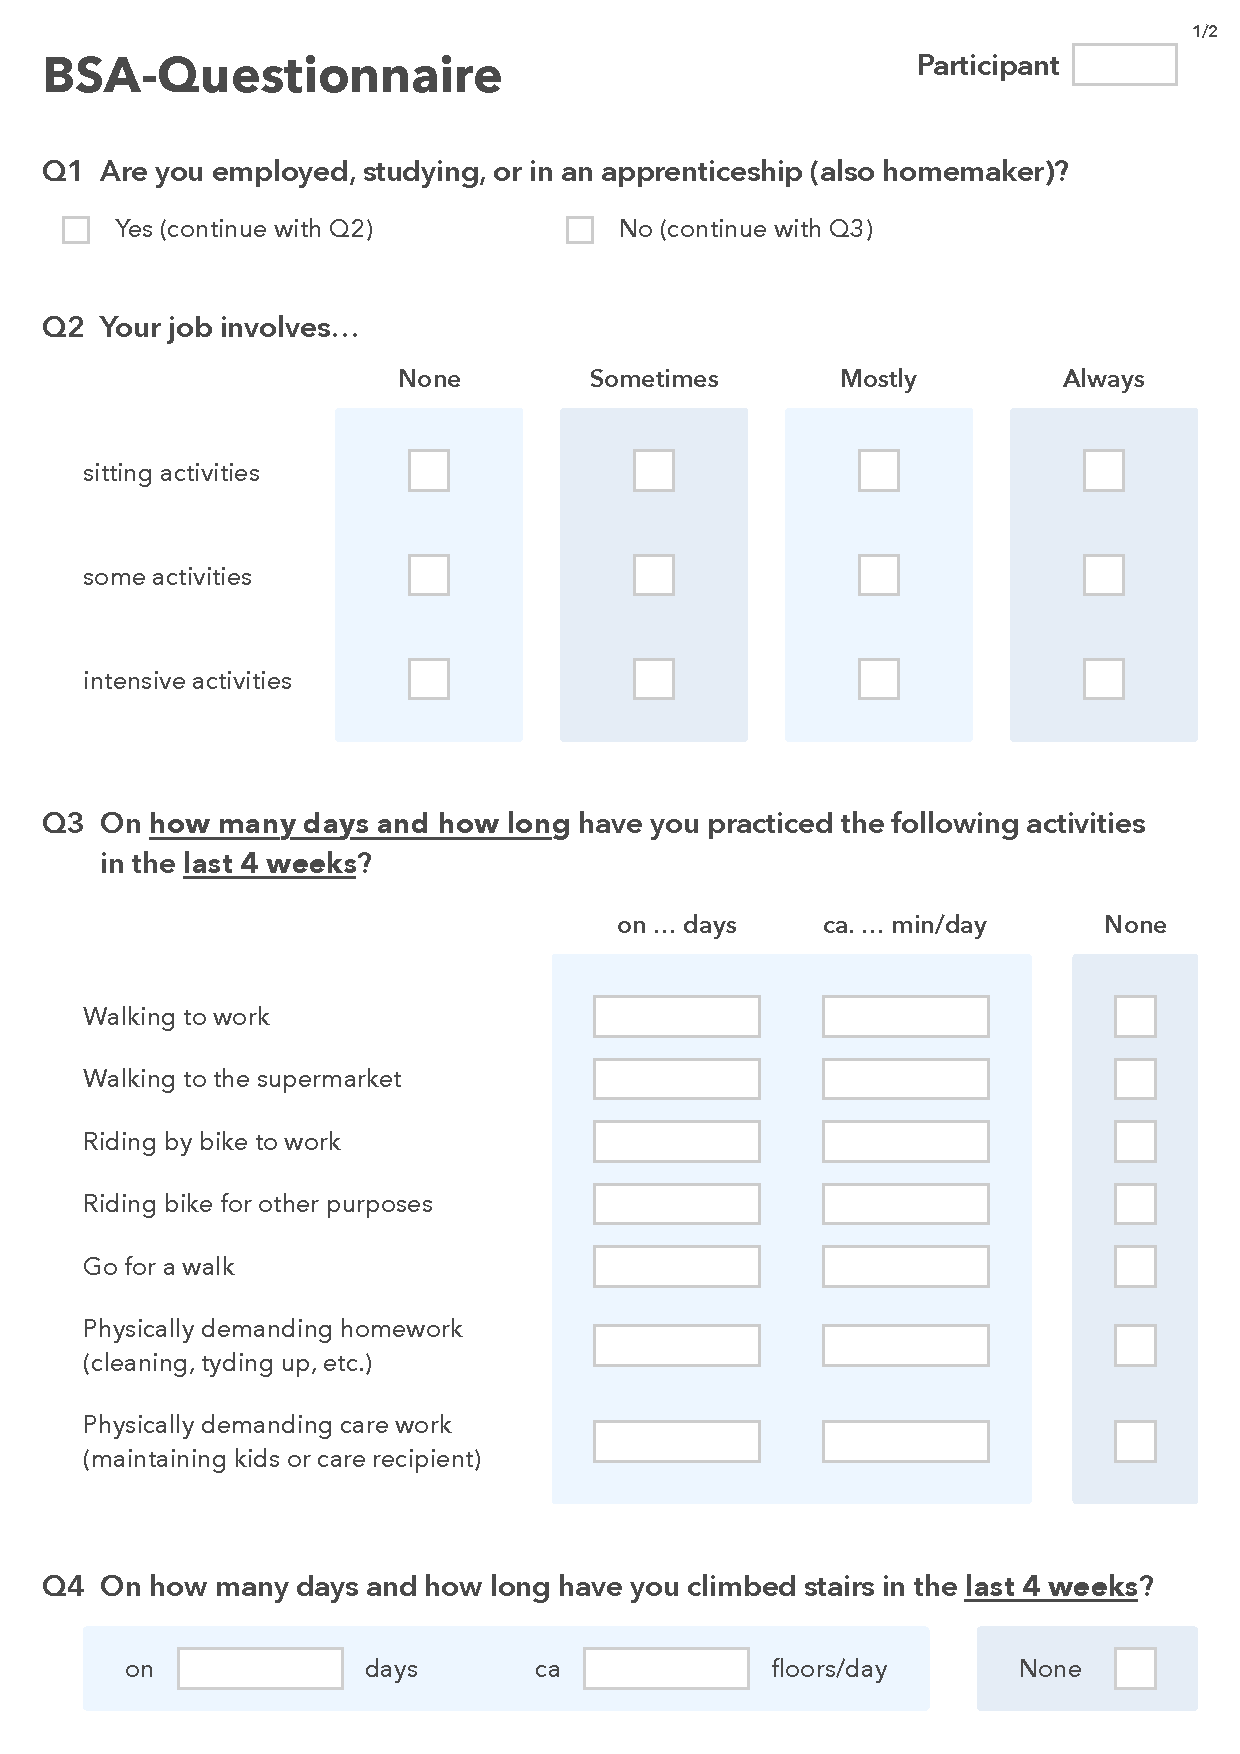
\includegraphics[width=1\linewidth]{Pictures/App_BSA-1}
		\caption{First page of the physical activity questionnaire, adapted from Fuchs et. al~\cite{Fuchs2015-bsa}}
		\label{fig:App_DemographicDataHTG}
	\end{minipage}
\end{figure}

\begin{figure}[htb]
	\centering
	\begin{minipage}[t]{1\linewidth}
		\centering
		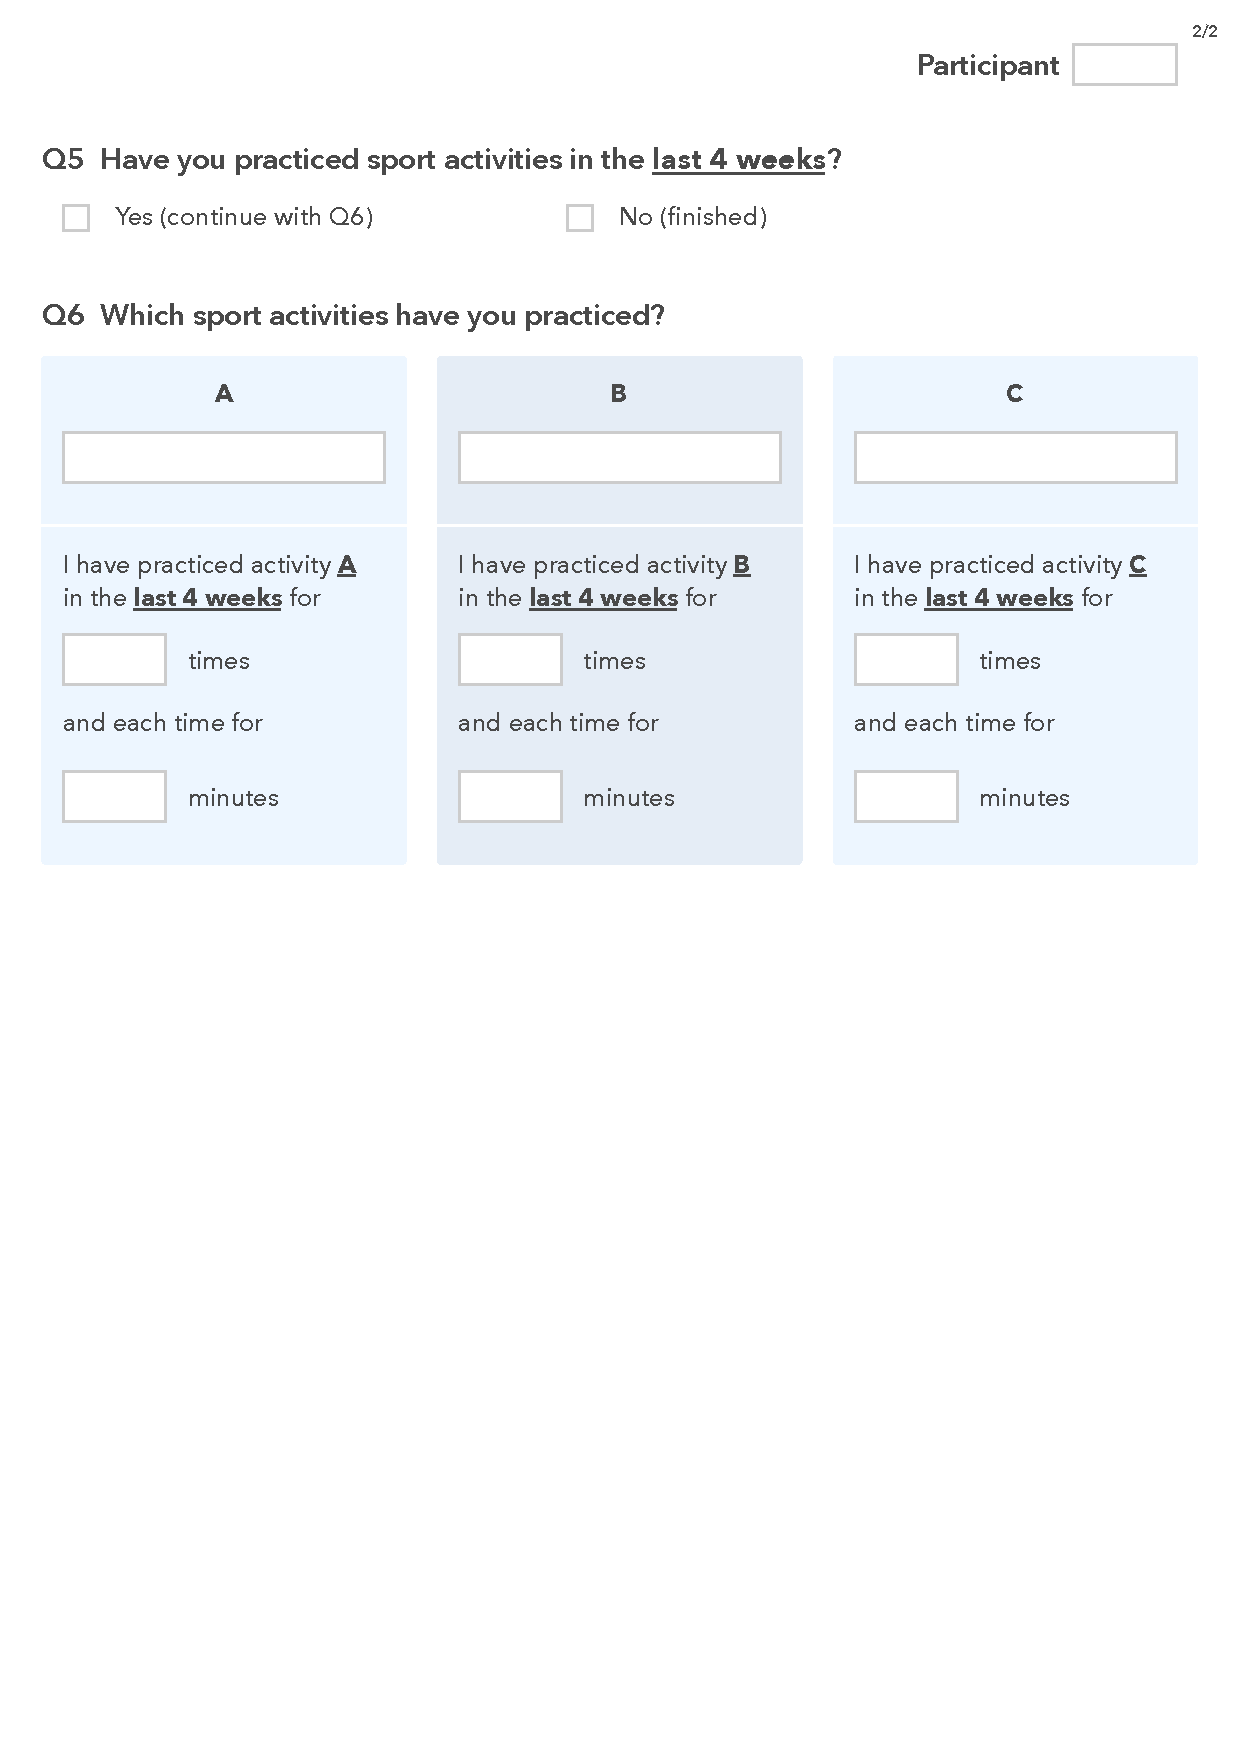
\includegraphics[width=1\linewidth]{Pictures/App_BSA-2}
		\caption{Second page of the physical activity questionnaire, adapted from Fuchs et. al~\cite{Fuchs2015-bsa}}
		\label{fig:App_DemographicDataHTG}
	\end{minipage}
\end{figure}

\clearpage

\begin{figure}[htb]
	\centering
	\begin{minipage}[t]{1\linewidth}
		\centering
		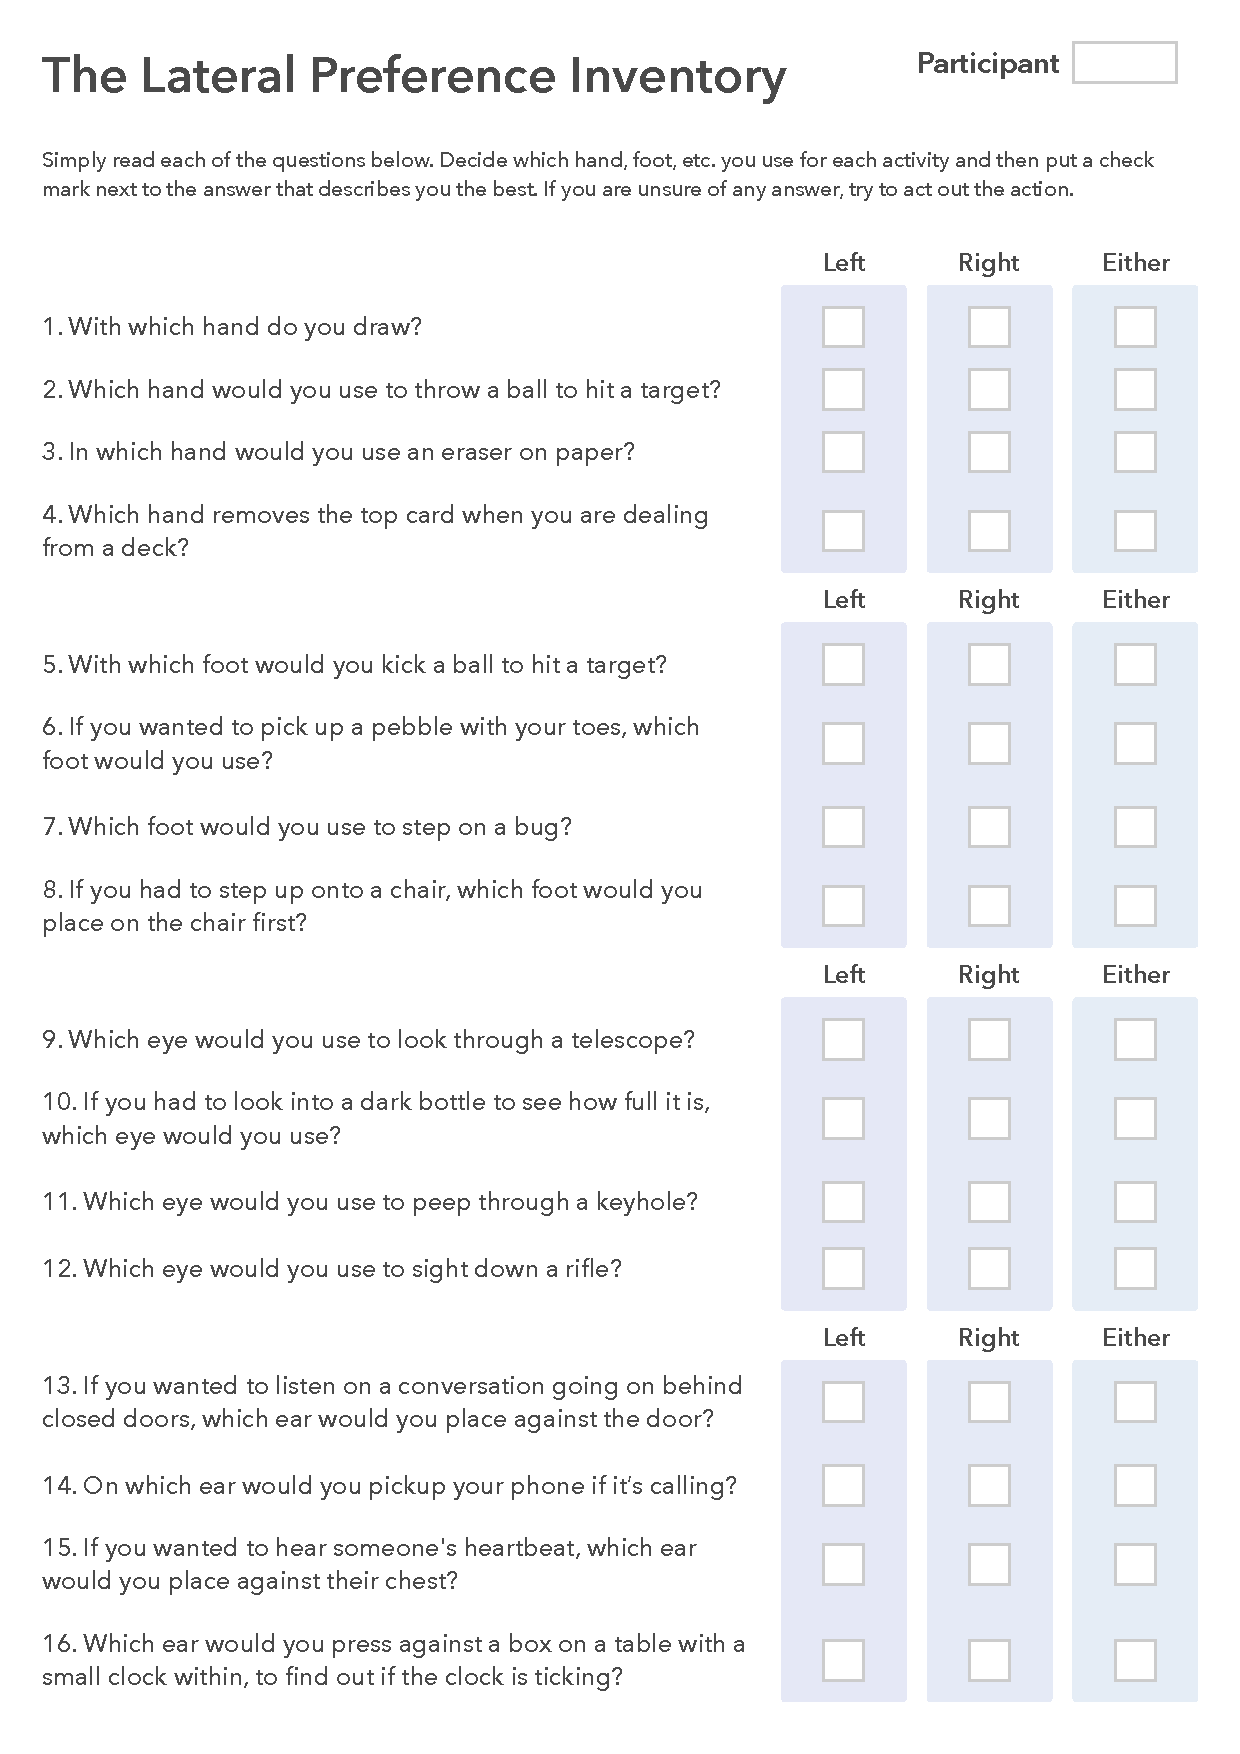
\includegraphics[width=1\linewidth]{Pictures/App_LateralPreference}
		\caption{Lateral preference inventory to determine the preference of the body side, adapted from Coren~\cite{Coren1993-lp}}
		\label{fig:App_DemographicDataHTG}
	\end{minipage}
\end{figure}

\clearpage

\section*{Guided Interview Questionnaire}

\subsection*{Block 1: General questions about the learning method}
Q1: How is your general experience about this training method?

Q2: What do you like the least?

Q3: What do you like the most?

Q4: Would you use this method and why?\\

\subsection*{Block 2: Application scenarios}
Q1: Could you think of any other application scenario for exactly this training method with the slacklining approach? (no hints but e.g. rehabilitation, sport medicine, etc.)

Q2: Could you think of any other sport activities, than slacklining, that could fit in this method?\\

\subsection*{Block 3: User Interface / System Feedback Evaluation~\footnote{These questions were just asked for the interactive system group}}
Q1: What do you like the most about the system?

Q2: What was most frustrating / disturbed you?

Q3: What would you change?

Q4: How would you describe the system in one sentence?

\chapter{Statement of the Ethical Review Board}
\begin{figure}[htb]
	\centering
	\begin{minipage}[t]{0.62\linewidth}
		\centering
		
\includegraphics[width=1\linewidth]{Pictures/App_EthicalReviewFeedback}
		\caption{Approvement of the Ethical Review Board in response to the research project}
		\label{fig:App_DemographicDataHTG}
	\end{minipage}
\end{figure}
\end{appendices}


\cleardoublepage
\markboth{List of Abbreviations}{List of Abbreviations}
\chapter*{List of Abbreviations}
\begin{acronym}
  \acro{3D}{\tab \\Three-Dimensional}
  \acro{CM}{\tab \\Centimetre}
  \acro{F}{\tab \\F-Ratio}
  \acro{HTG}{\tab \\Human Trainer Group}
  \acro{ISG}{\tab \\Interactive System Group}
  \acro{M}{\tab \\Metre}
  \acro{P}{\tab \\Asymptotic Significance}
  \acro{PC}{\tab \\Personal Computer}
  \acro{SEC}{\tab \\Seconds}
  \acro{SDK}{\tab \\Software Development Kit}
  \acro{SLS}{\tab \\Slackline Learning System}
  \acro{UI}{\tab \\User Interface}
  \acro{VGB}{\tab \\Visual Gesture Builder}
\end{acronym}
\addcontentsline{toc}{chapter}{\hspace {-6mm}List of Abbreviations}

\cleardoublepage
\listoffigures
\addcontentsline{toc}{chapter}{\hspace {-6mm}\listfigurename}

\cleardoublepage
\listoftables
\addcontentsline{toc}{chapter}{\hspace {-6mm}\listtablename}

\clearpage
\begingroup
  \pagestyle{plain}
  \bibliographystyle{acm_fkerber}
   \phantomsection
	\bibliography{references}\emph{}
	\addcontentsline{toc}{chapter}{\hspace {-6mm}Bibliography}
	\vfill
  \clearpage
\endgroup 
\end{document}